\ifx\allfiles\undefined
\documentclass[12pt, a4paper, oneside]{ctexbook}
%\usepackage{microtype}
\usepackage{amsmath, esint,amsthm, amssymb, bm, color, framed, graphicx, imakeidx, geometry,
hyperref, mathrsfs,lipsum,fancyhdr,indentfirst,array,tabularx,float,prettyref,stmaryrd}
%文内引用
%插入书签:\label{myref:引用内容(英文字母,中文出现了编译错误)}
%引用书签:\prettyref{myref:引用内容}

\allowdisplaybreaks[4]

%简化的指令
%\renewcommand{\i}{\mathrm{i}}%虚数i
\newcommand{\di }{\text{d}}%微分
\newcommand{\pian }{\partial}%偏导数
\newcommand{\die }{\textbf{d}}%外微分
\newcommand{\fuyi }{^{-1}}%逆映射
\newcommand{\card }{\text{card}}%势
\newcommand{\R }{\mathbb{R}}%实数
\newcommand{\Z }{\mathbb{Z}}%整数
\newcommand{\RR }{$\R\ $}%实数(文本)
\newcommand{\Rn }{$\R^n\ $}%实数(文本)
\newcommand{\N }{\mathbb{N}}%自然数
\renewcommand{\S}{\mathcal{S}}%S
\newcommand{\fai }{\varphi}%常用的那个小phi
\newcommand{\e }{\vec{e}}%向量e
\newcommand{\Id }{\text{Id}}%单位元
\newcommand{\continue }{\text{连续}}%连续
\newcommand{\C }{\mathcal{C}}%连续函数类
\newcommand{\Com }{\mathbb{C}}%复数
\newcommand{\M }{\mathcal{M}}%矩阵
\newcommand{\Hess }{\text{Hess}}%Hess矩阵
\newcommand{\normmm}[1]{{\left\vert\kern-0.25ex\left\vert\kern-0.25ex\left\vert #1 
   \right\vert\kern-0.25ex\right\vert\kern-0.25ex\right\vert}}%|||v|||三个竖线的范数
%常用的文本里的字母
\newcommand{\x }{$x$}\newcommand{\xo }{$x_0$}
\newcommand{\y }{$y$}\newcommand{\yo }{$y_0$}
\newcommand{\z }{$z$}\newcommand{\zo }{$z_0$}
\newcommand{\n }{$n$}\newcommand{\f  }{$ f $}

\title{
\vspace{-2cm}
  \begin{figure}[!t]%插入题目的图片
    \centering
    
\includegraphics[width=14cm]{shulijichu-2.png}
  \end{figure}
  \vspace{-2cm}
  {\Huge{\textbf{工程师学院数学理论基础\\
Fondements des Théories Mathématiques de l'Ecole d'Ingénieur de Chimie Pékin\\
第一部分:基础知识\\
Partie I: Notions Élémentaires
}}}
}
\author{Augustin}
\date{最后更新于:\today}
\linespread{1.5}
\makeindex

\setcounter{tocdepth}{1}%两个2说明只显示到subsection
\setcounter{secnumdepth}{2}

%\def\allfiles{}
\begin{document}
\newrefformat{myref}{第\ref{#1} 节}
\vspace{-3cm}
\maketitle
\tableofcontents
\else
\part{基础知识\\ Notions Élémentaires}
\fi
%开始本部分正文
\chapter{逻辑与证明\\ Logique et Démonstration}
  这一章内容是数学最基本的、最底层的概念.对于绝大多数阅读这份讲义的人而言,前几节的东西都已经学习过了,或者显而易见的.
  但这并不意味着这一章的内容就很好写,或者很好讲明白.也因此,为了保持知识的丰富度和连贯性,有许多还没在本讲义里被严格定义,但是其实已经学过的知识会出现在本章(后面也是).
  对于绝大多数这类情况,并不存在阅读障碍.但是,如果你发现有什么地方不太对劲,或者有什么地方不太懂,欢迎联系我,我会尽快修改.\\


  这一章(以及后面的章节里)有相当多的符号,关于这些符号的采用和相关的历史,欢迎参阅\url{https://jeff560.tripod.com/set.html}.
  \section{基本逻辑 Basic Logique}
  
  \subsection{命题逻辑 Logique propositionnelle}
  命题(Proposition)是一个陈述句所表达的判断,不是真的就是假的.例如“我不懂数学”就是一个命题.当然,在本讲义中,带有Proposition节标题的内容都被认为是真的.
  \subsubsection{逻辑析取:或  la disjonction: ou}
  定义符号 $\lor $ 表示两个命题的逻辑析取.对于命题$p,q,\text{若}p$是真的或者$q$是真的,则$p\lor q$是真的.
  \subsubsection{逻辑合取:与  la conjonction: et }
  定义符号 $\land  $ 表示两个命题的逻辑合取.对于命题$p,q,\text{若}p$和$q$都真的,则$p\land q$是真的.
  \subsubsection{逻辑否定:非  la négation: non}
  定义符号 $\lnot $ 表示命题的逻辑否定.若命题$p$是真的,则$\lnot(p)$是假的.
  \subsubsection{逻辑蕴含 l'implication}
  定义符号 $\Rightarrow$ 表示两个命题的逻辑蕴含.对于命题$p,q$,将$p\lor(\lnot q)$记为$q\Rightarrow p$.
  表示若$q$是真的则$p$也是真的.注意,如果$p,q$都不是真的,$q\Rightarrow p$也是真的.
  \subsubsection{逻辑等价 l'équivalence}
  定义符号 $\Rightarrow$ 表示两个命题的逻辑等价.对于命题$p,q$,将$(p\Rightarrow q)\land (q\Rightarrow p)$记为$p\Leftrightarrow q$.
  称作p等价于q.
  \subsection{逻辑公理 Axiomes de la logique}
  公理被认为是清晰地为真的命题.以下给出逻辑的四条公理.
  \subsubsection{$AL_1$}
  $(p\lor p)\Rightarrow p$是真的.这说明,如果$(p\lor p)$为真,则$p$为真.
  \subsubsection{$AL_2$}
  $p\Rightarrow (p\lor q)$是真的.这说明,如果$p$为真,则$(p\lor q)$为真.
  \subsubsection{$AL_3$}
  $(p\lor q)\Rightarrow (q\lor p)$是真的.这说明,如果$(p\lor q)$为真,则$(q\lor p)$为真.
  \subsubsection{$AL_4$}
  $(p\Rightarrow q)\Rightarrow [(p\lor r)\Rightarrow(q\lor r)]$是真的.
  \subsection{De Morgan定律 Lois de De Morgan}\index{De Morgan 定律}
  数学家Augustus De Morgan发现了命题逻辑中存在着如下关系:
  \begin{itemize}
    \item $\lnot (p\wedge q)\equiv (\lnot p)\vee (\lnot q) $
    \item $\lnot (p\vee q)\equiv (\lnot p)\wedge (\lnot q) $
  \end{itemize}称为De Morgan定律,又叫对偶律.

  \subsection{量词 Quantificateur}
  \subsubsection{全称量词 Quantification Universelle}
  全称量词$\forall$表示“对所有的(pour tout)”.由Gerhard Gentzen首先于1933年使用,将德语“一切(alle)”的首字母倒过来.

  \subsubsection{存在量词 Quantification Existentielle}
  存在量词$\exists$表示“存在(il existe)”.由Giuseppe Peano首先于1897年使用,后被Bertrand Arthur William Russell正式用于表示“存在”.
  此外,存在量词$\exists !$表示“有且仅有唯一的(il existe et seul)”.

  \section{证明 Démonstration}
  给定命题$p$,现在并不清楚命题是真是假.如果我们想要命题为真,就需要从逻辑上证明.同理,如果想要为假,也要从逻辑上证伪.这些都属于证明.
  \subsection{逻辑变换 Transformations logiques}
  蕴含命题$p\Rightarrow q$,全称命题$\forall x,p(x)$和存在命题$\exists x,q(x)$有如下的逻辑变换:
  \subsubsection{逆命题 Implication Réciproque}
  蕴含命题$p\Rightarrow q$的逆命题为$q\Rightarrow p$,逆命题不受量词影响,即$\forall x,p(x)\Rightarrow q(x)$的逆命题为$\forall x,q(x)\Rightarrow p(x)$.
  \subsubsection{否命题 }
  蕴含命题$p\Rightarrow q$的否命题为$\lnot p\Rightarrow \lnot q$.
  全称命题$\forall x,p(x)$的否命题为$\exists x,\lnot p(x)$,
  存在命题$\exists x,q(x)$的否命题为$\forall x,\lnot q(x)$.
  \subsubsection{逆否命题 Proposition Contraposée}
  蕴含命题$p\Rightarrow q$的逆否命题为$\lnot q\Rightarrow \lnot p$.逆否命题与原命题等价.
  \subsection{三段论 Syllogisme}
  三段论是涉及三个命题的论证,形式如$[(A\Rightarrow B)\land (B\Rightarrow C)]\Rightarrow (A\Rightarrow C)$.
  一般而言,一个三段论分为大前提(Prémisse majeure),小前提(Prémisse mineure)和结论(Conclusion)三段.
  大前提是某种普遍性质的规律,小前提是一个特殊陈述,结论就是我们要证明的内容.
  例如要证明114是偶数,我们需要:\begin{itemize}
    \item 大前提:能整除2的数是偶数.
    \item 小前提:114能整除2.
    \item 结论:114是整数.
  \end{itemize}
  三段论的每段共有四种含义,分别为:
  \begin{itemize}
    \item A:$\forall s,p(s)$.例如:所有自然数都是实数.
    \item E:$\forall s,\lnot p(s)$.例如:所有自然数都不是负数.
    \item I:$\exists s,p(s)$.例如:存在实数是自然数.
    \item O:$\exists s,\lnot p(s)$.例如:存在实数不是自然数.
  \end{itemize}
  因此一个三段论可以被简写称诸如AAA或者AEO这样的形式,共计256种!然而只有24种是有效的.在这里我就不一一列出了,有兴趣的读者自行查阅相关内容.
  下面我们直接介绍具体的证明方法.当然,如果你能将证明方法与对应的三段论结构联系起来,那是非常棒的!

  \subsection{举例证明 Preuve par exemple}
  假设要证明命题“存在不可导连续函数”,我们只需要举出一个例子就行,比如绝对值函数$f(x)=|x|$.
  同理,证伪命题“所有连续函数都可导”也是这样.
  \subsection{逆否证明 Preuve par contraposée}
  逆否命题与原命题等价,因此只需证明或者证伪逆否命题,就能间接证明或证伪原命题.
  \subsection{反证法 Preuve par l'absurde}
  假设我们要证明命题A为真,我们可以假设$\lnot $A为真,然后推出一个矛盾的结果$\perp $,因此$\lnot $A为假,从而证明A为真.\\
  
  
  例如,我们要证明素数有无限个.采用反证法:$\lnot(\text{素数有无限个})\Rightarrow \text{素数有有限个} $.设全体素数组成的集合$\mathbb{P}=\{p_1,p_2,\dots,p_n\}$,
  设$n=1+\prod _{i=1}^{n}p_1$,显然$n\notin \mathbb{P}$.若\n 是素数,则我们得到了一个不属于全体素数集合的素数,这显然矛盾.若\n 不是素数,对其质因数分解,选择任意一个质因子$m$.
  若$m\in \mathbb{P}$,则$m$既是$1+\prod _{i=1}^{n}p_1$的因子,又是$\prod _{i=1}^{n}p_1$的因子,因此必须是两者之差1的因子,也就是1.因此$n=m\cdot 1$,\n 显然是素数,
  所以我们又得到了矛盾的结果.所以,只能是我们的前提“素数有有限个”是错的,故素数有无限个.
  \subsection{归纳法 Preuve par récurrence}
  
  \subsection{分类讨论 Preuve par cas}



  
  更多关于证明的例子和技巧,可以参阅roofs from THE BOOK这本书(中文名叫《数学天书中的证明》),其涵盖了数论、几何、分析、组合数学和图论的许多精美的证明.

  \section{严格逻辑公式 Formules strictes}
  通过以上的逻辑符号和公理,加上两个用于判断的符号 $\perp $ 表示"假"和 $\top $ 表示"真",我们可以构造出一些严格逻辑公式.
  \subsection{Définition: Formule stricte}
  严格逻辑公式的定义实际上是一种归纳法.
  \begin{enumerate}
    \item $\perp $ 和 $\top $ 是严格逻辑公式.
    \item 任意的变量都是严格逻辑公式.
    \item 对任意严格逻辑公式$A$, $\lnot A$也是严格逻辑公式.
    \item 对任意两个严格逻辑公式$A$和$B$, $(A\land B)$,$(A\lor B)$,$(A\Rightarrow B)$,$(A\Leftrightarrow B)$也是严格逻辑公式.
  \end{enumerate}
  在一些推理中,利用$\circ$代表$\land,\lor,\Rightarrow,\Leftrightarrow$中的任意一个,并将 formule stricte 简称为逻辑公式 formule.
  此外,对于除了$\perp $和$\top $以外的逻辑公式,我们称其为可分解的(décomposable).
  \subsubsection{Exemple}
  $(a\lor(\lnot b\land c))$是逻辑公式,但是$a\lor(\lnot b\land c)$和$(a\lor(\lnot( b)\land c))$不是.
  \subsection{Définition: 子公式 Sous-formule stricte}
  称(严格)公式 $A$ 的任何因子为$A$的子公式.例如$(\lnot b\land c)$是$(a\lor(\lnot b\land c))$的子公式.
  \subsection{Définition: 公式的长度 Longueur d'une formule}
  公式 $A$ 的长度是用于编写 $A$ 的符号数量,用 $l(A)$ 表示.
  如果我们将公式视为用词汇表中的元素构成的词,其中的元素包括常量、变量、括号和连接符.
  则在这个词汇表上的一个词是该词汇表中元素的一个序列,而该词的长度是该序列的长度.
  例如$A=(a\land b)$,$B=(A\lor \lnot A)$,则$l(A)=5,\,l(B)=4+5+5=14$.
  \subsection{Définition: 公式的前缀 Préfixe d'une formule}
  对任意公式$A$,其前缀(préfixe)是从该公式的开头一直延伸到某个位置的部分.
  这个位置可以是一个特定的字符,一个操作符或一个括号,用来截断公式的前缀.
  例如$($和$(a$都是$A=(a\land b)$的前缀.但是$)$或者$b)$不是.
  此外,对于长度严格小于$A$的前缀,我们称其为严格前缀(préfixe strict).
  \subsection{括号的平衡  Équilibre des parenthèses}
  任何公式都具有相等数量的开括号"$($"和闭括号"$)$".可直接由定义和归纳法得到.
  \subsection{括号的关联 Relation entre les parenthèses}
  任何公式的前缀都具有至少与闭括号相等数量的开括号.
  \subsubsection{Démonstration}
  首先假设对于任意长度小于$n$的公式,该定理都成立。接着假设$l(A)=n$.
  \begin{enumerate}
    \item 若$A$是一个变量或者常量,则$A$没有括号,因此该定理成立.
    \item 若$A=\lnot B$,则$A$的前缀要么是空的或者$\lnot$,要么是$\lnot$跟随$B$的前缀,而$l(B)<n$,因此该定理成立.
    \item 若$A=(B\circ C)$,则$A$的前缀要么是空的或者开括号,要么是开括号跟随$B$的前缀,要么是开括号跟随$B\circ$和$C$的前缀.根据以上结论,都满足该定理.
  \end{enumerate}
  因此,如果引理对于所有长度小于$n$的公式都成立,那么它也对于长度为$n$的任何公式成立。
  通过归纳法,我们可以得出它对于任何长度的公式都成立。
  这个证明证明了数学逻辑中公式的括号平衡性质。
  \subsection{Définition: 公式的大小 Taille d'une formule}
  对公式$A$定义$|A|$为:
  \begin{itemize}
    \item 若$A$是$\perp$或$\bot$,则$|A|=0$.
    \item 若$A$是变量,则$|A|=0$.(?)
    \item $|\lnot A|=1+|A|$.
    \item $|A\circ B|=1+|A|+|B|$.
  \end{itemize}
  \subsection{严格前缀引理 Lemme des préfixes stricts}
  任何公式的严格前缀不是一个公式.\\
  Tout préfixe strict d'une formule n'est pas une formule.
  \subsubsection{Démonstration}
  仍然采用归纳法.对于基本情况$|A|=0$,$A$要么是变量要么是常量,其严格前缀只能是空的,故不是公式.
  假设对于任意长度小于$n$的公式,该定理都成立。接着假设$|A|=n$.

  若$A=\lnot B$,则$A$的严格前缀要么是空的或者$\lnot$,要么是$\lnot$跟随$B$的严格前缀,而$|B|<n$,因此该定理成立.

  若$A=(B\circ C)$,假设$A$有一个为公式的严格前缀$A_0=(B\circ C_0)$,其中$C_0$是$C$的前缀.
  为了保持公式的开括号与闭括号数量一致,我们必须有$C_0=C$.因此$A_0=A$,与严格前缀矛盾.因此该定理成立.
  \subsection{Proposition}\label{myref:sixuanyi}
  对于任何公式$A$,其有且仅有可能为以下形式之一:
  \begin{itemize}
    \item $A$是一个变量
    \item $A$是一个常量
    \item $A=\lnot B$,其中$B$是一个公式,且$A$是唯一的
    \item $A=(B\circ C)$,其中$B,C$是公式,且$A$是唯一的
  \end{itemize}
  \subsubsection{Démonstration}
  事实上我们只需证明最后一种形式.同样可以假设$A=(B\circ C)=(B_0\circ C_0)$然后证明$B_0=B,\,C_0=C$.与之前没什么差别.
  \subsection{优先级 Priorité}
  在定义公式时,我们写了很多不必要的括号,例如每个公式周围的括号。现在,我们通过定义优先级为语法引入了更多的灵活性。
  同样利用归纳法定义具有优先级的公式(或称为优先级公式 formule à priorité):
  \begin{itemize}
    \item $\perp $ 和 $\top $ 是优先级公式.
    \item 任意的变量都是优先级公式.
    \item 对任意优先级公式$A$, $\lnot A$也是优先级公式.
    \item 对任意两个优先级公式$A$和$B$, $A\circ B$也是优先级公式.
    \item 对任意优先级公式$A$, $(A)$也是优先级公式.
  \end{itemize}
  例如$a\lor \lnot b\land c$是一个优先级公式,但它并不是公式.为了确保公式的唯一性,我们需要定义连接词的优先级顺序.
  \subsubsection{优先级顺序 Ordre de priorité des connecteurs}
  定义连接词的优先级顺序(由高到低)如下:
  \begin{enumerate}
    \item $\lnot$ 否定 la négation
    \item $\land$ 合取 la conjonction
    \item $\lor$  析取 la disjonction
    \item $\Rightarrow$ 蕴含 l'implication
    \item $\Leftrightarrow$ 等价 l'équivalence
  \end{enumerate}
  \subsubsection{Remarque}
  在相同优先级的情况下,左侧的连接词具有更高的优先级,但对于蕴含操作符,它是右结合的。
  我们将一个具有优先级的公式视为使用优先级可重新构建的公式的缩写。
  除非另有说明,我们将一个公式与其缩写视为相同。
  换句话说,我们关注的是一个公式的结构,而不是它的表面写法,这一结构通过"stricte"语法得以明确。
  因此,具有优先级的公式的大小将等于它所代表的严格公式的大小。
  \section{公式的意义 Sens des formules}
  在这一部分,我们将探讨如何确定一个公式的真假,而不依赖于为其变量分配的值。
  我们首先会定义逻辑连接词的含义,然后解释如何计算一个公式的真值,并展示紧凑性定理。
  最后,我们将介绍逻辑学中的基本概念定义,这些构成了逻辑学家们的通用语言。
  \subsection{连接词的真假 Valeur de vérité des connecteurs}
  通常用0表示值为假,用1表示值为真.这样,可以分别依据变量$x$和$y$的真假给出连接词的真假.
  \begin{table}[H]
    \centering
  \begin{tabular}{|c|c|c|c|c|c|c|}
    \hline
    $x$ & $y$ & $\neg x$ & $x \lor y$ & $x \land y$ & $x \Rightarrow y$ & $x \Leftrightarrow y$ \\\hline
    0 & 0 & 1 & 0 & 0 & 1 & 1 \\\hline
    0 & 1 & 1 & 1 & 0 & 1 & 0 \\\hline
    1 & 0 & 0 & 1 & 0 & 0 & 0 \\\hline
    1 & 1 & 0 & 1 & 1 & 1 & 1 \\\hline
    \end{tabular}
    \caption{连接词真值表 Table de vérité des connecteurs}
    \label{tab:connecteurs}
  \end{table}
  \subsection{公式的值 Valeur d'une formule}
  我们为公式中的每个变量分配一个来自集合 $B = \{0, 1\}$ 的值。
  公式的值通过将变量替换为它们的值并根据表\ref{tab:connecteurs}的操作来计算得到。
  然而,为了对公式进行推理,我们需要正式定义公式的值。
  \subsubsection{Définition: 赋值 Assignation}
  赋值是将公式中的所有变量映射到集合$B$中.

  Une assignation est une application de l'ensemble de toutes les variables d'une formule dans l'ensemble $B$.
  \subsubsection{Définition: 公式的值 Valeur d'une formule}
  对于一个公式$A$和一个赋值$v$,我们定义$A$在$v$下的值$[A]_v$如下,其中$A,B$是公式,$x$是变量,$v$是赋值.
  \begin{itemize}
    \item $[x]_v=v(x)$
    \item $[\bot]_v=1,\,[\perp]_v=0$
    \item $[\lnot A]_v=1-[A]_v$
    \item $[A\land b]_v=\max\{[A]_v,[B]_v \}$
    \item $[A\lor b]_v=\min\{[A]_v,[B]_v \}$
    \item $[A\Rightarrow b]_v=\begin{cases}
      1 & [A]_v=0\\
      [B]_v & [A]_v\neq 0
    \end{cases}$
    \item $[A\Leftrightarrow b]_v=\begin{cases}
      1 & [A]_v=[B]_v\\
      0 & [A]_v\neq [B]_v
    \end{cases}$
  \end{itemize}
  根据\prettyref{myref:sixuanyi}的结论,根据第14页的定理1.1.13,每个严格的公式都可以唯一分解为上述情况之一。
  这意味着将变量的赋值扩展到所有公式是一个从公式到B的映射。
  例如,对于四个公式 $A$、$A_0$、$B$ 和 $B_0$ 以及两个操作符 $\circ$ 和 $\circ_0$,
  如果 $(A\circ B)=(A_0\circ_0 B_0)$,则根据分解的唯一性,我们可以得出 $A=A_0$,$B=B_0$,$\circ=\circ_0$。
  因此,公式 $(A\circ B)$ 的值仅由值定义中的一行唯一确定。这表明公式的值仅与其包含的变量和结构有关,因此公式的计算以真值表的形式展示,如表\ref{tab:formes}所示.
  \begin{table}[ht]
    \centering
    \begin{tabular}{|c|c|c|c|c|c|c|}
      \hline
      $x$ & $y$ & $\neg x$ & $x\lor y$ & $x\land y$ & $x\Rightarrow y$ & $x\Leftrightarrow y$ \\\hline
      0 & 0 & 1 & 0 & 0 & 1 & 1 \\\hline
      0 & 1 & 1 & 1 & 0 & 1 & 0 \\\hline
      1 & 0 & 0 & 1 & 0 & 0 & 0 \\\hline
      1 & 1 & 0 & 1 & 1 & 1 & 1 \\
      \hline
    \end{tabular}
    \caption{公式真值表 Table de vérité des formules suivantes}
    \label{tab:formes}
  \end{table}

  \section{替换和取代 Substitution et remplacement}
  \section{标准形式 Formes normales}
  将一个公式转化为标准形式是将其转化为一个具有结构性质的等价公式的过程。
  我们引入了两种标准形式的概念:析取范式(Disjunctive Normal Form,DNF),用于突出模型,
  以及合取范式(Conjunctive Normal Form,CNF),用于展示反例。
  标准形式的定义需要引入文字(literal)、单项式(monomial)和子句(clause)的概念。


  \section{Boole代数 Algèbre de Boole}
  \section{Boole函数 Fonctions booléennes}
  \section{二进制决策图计算器 Binary Decision Diagram based Calculator}
\section{一阶逻辑 Logique du premier ordre}
  待修改






\chapter{集合\\ Ensembles}
  我们先从数学最基础的内容开始.前面这一部分内容在大一就已经讲过了,然而为了保持本讲义的连贯与严谨,不突兀地出现公理化集合论之类的东西,我们还是从头开始讲起.
\section{集合}
  为了便于你的理解,我们先给出集合的定义,并且顺着这些定义讨论,随后会在\prettyref{myref:gonglihua}这里把这些概念全部公理化,以求得到更深刻的理解.
  事实上,本讲义的许多内容,都是先讲个基础的概念,随后在某个内容里将这个概念公理化.
  \subsection{Définition}
  我们朴素地认为,一个集合就是将对象归类而分成为一个或数个形态各异的大小整体.
  一般来讲,集合是具有某种特性的事物的整体,或是一些确认对象的汇集.构成集合的事物或对象称为元素.集合的元素可以是任何东西.
  \subsection{集合的特性}
  集合具有以下几个特性:
  \begin{itemize}
    \item 无序性:一个集合中,每个元素的地位都是相同的,元素之间是无序的.\footnote{
      当然,如果我们在集合上定义了序,那么元素之间就可以按照序关系排序.但就集合本身的特性而言,元素之间没有必然的序.序关系将在后续阐明.
    }
    \item 互异性:一个集合中,每个元素只能出现一次,没有相同的元素出现.
    \item 确定性:给定一个集合,任给一个元素,该元素或者属于或者不属于该集合.\label{myref:quedingxing}
  \end{itemize}
  \subsection{索引族 Famille Indexée}
  若集合$I$中的每个元素,比如$i$,都对应着一个集合$A_i$,那么称$\mathscr{A}=\{A_i|i\in I\}$为集合$A$的索引族,集合$I$是其索引集.
  \subsubsection{Exemple}
  $A_n=\{1,14,n^2\}$,且有$\mathscr{A}=\{A_n|n\in [\![5,14]\!]\}$,则$\mathscr{A}$就是$A_n$的索引族,并且$\mathscr{A}=\{ \{1,14,25\}\{1,14,36\}\dots\{1,14,196\}\}$.
  \subsection{子集 Sous-ensemble}
  若集合$B$中的每个元素都属于集合$A$,则集合$B$是集合$A$的子集,则集合$A$是集合$B$的超集,记为$B\subseteq A$或者$A\supseteq B$.
  此外,若$B\subseteq A$且$A\subseteq B$,说明二者的元素相同,是同一个集合,记为$A=B$.
  \subsubsection{Proposition}
  对于任意集合$A$,有$\varnothing\subseteq A$.
  \subsection{幂集 Ensemble Puissance}
  对于任意集合$A$,其幂集为由该集合全部子集为元素构成的集合,记为$\mathcal{P},\mathcal{P}(A)=\{B| B\subseteq A\}$.
  有时也称之为ensemble des parties.

  \section{二元关系 Relation Binaire}
  \subsection{有序对 Couple}
  有序对是包含了两个元素的特殊的集合$(a,b)$.不同于一般的集合,有序对上的两个元素是有顺序的,
  分别被称为左投影和右投影,法语也叫première composante和deuxième composante.有序对的相等要求:
  $$
  (a_1,b_1)=(a_2,b_2)\Leftrightarrow (a_1=a_2)\land(b_1=b_2)
  $$有序对可以有其他有序对作为投影,所以有序对使得能够递归定义有序.
  例如,有序三元组 (a,b,c)可以定义为(a, (b,c)),一个对嵌入了另一个对.
  \subsection{Définition}
  二元关系将一个集合的元素与另一个集合的元素相关联.例如集合$X$和$Y$上的二元关系$\mathcal{R} $是一组新的有序对$(x,y)\text{组成的集合$\mathcal{G} $,其中}x\in X,y\in Y$.
  如果$(x,y)\in\mathcal{G}$,则称$x,y$有关系$\mathcal{R}$,记作$x\mathcal{R}y$或者$\mathcal{R}(x,y)$.
  \subsubsection{Exemple}
  $\mathbb{N}$上的大于关系$>$可以表示为$\{(a,b)|\exists r\in \mathbb{N},(a=b+r)\}$.记作$a>b$.
  \subsection{关系的性质}
  二元关系$R$可能拥有以下的某些性质:
  \subsubsection{自反性 Relation Réflexive}
  $\forall x\in X,(x,x)\in R$
  \subsubsection{非自反性 Relation Irréflexive}
  $\forall x\in X,(x,x)\notin R$
  \subsubsection{对称性 Relation Symétrique}
  $\forall x\in X,y\in Y,(x,y)\in R\Leftrightarrow(y,x)\in R$
  \subsubsection{反对称性 Relation Antisymétrique}
  $\forall x\in X,y\in Y,(x,y)\in R\land(y,x)\in R \Leftrightarrow x= y$
  \subsubsection{非对称性 Relation Asymétrique}
  $\forall x\in X,y\in Y,(x,y)\in R\Rightarrow (y,x)\notin R$
  \subsubsection{传递性  Relation Transitive}
  $\forall(x,y)\in R,\forall (y,z)\in R\Rightarrow(x,z)\in R$
  \subsection{等价关系 Relation d'Équivalence}
  若二元关系$\thicksim $满足自反性、传递性和对称性,则称其为等价关系,记作$a\thicksim b$.
  \subsubsection{Exemple}
  \begin{itemize}
    \item 集合的相等是等价关系.
    \item 三角形的相似关系和全等关系是等价关系.
    \item 温度相同是等价关系.
  \end{itemize}
  \subsubsection{等价类 Classe d'Équivalence}
  集合$E$上定义等价关系$\thicksim $,对$a\in E$,$a$的等价类为集合中所有与其等价的元素组成的集合$\{x|x\thicksim a\land x\in E\}$.
  
  \subsection{序关系 Relation d'Ordre}
  前文说过,集合上的元素本身是无序的,这意味着元素之间是平等的,无法比较的.
  例如给定集合$\{$2000CNY,3000USD,1919JPY,400EUR$\}$,我们并不知道四个元素分别意味着什么,也不知道他们的关系.现在给出 $Champion$ 断言: 2000CNY$\ge$3000USD.
  为什么可以这么说?显然,这说明存在某种“顺序”,这种“顺序”可以通过符号$\ge$来表示两个元素的关系.事实上,这就是一种序关系.下面我们分别介绍各种序关系.
  \subsubsection{全序关系 Relation d'Ordre Total}
  若集合$X$上的关系$\leq$满足自反性、传递性和反对称性,并且是“完全的(Totalité)”,也就是$\forall a\in X,\forall b\in X,(a\leq b)\lor(b\leq a)$.
  则称此关系为全序关系,或者非严格全序关系.\\
  
  相对应的,若集合$X$上的关系$<$定义为$a<b\Leftrightarrow \lnot(b\leq a)$,则称为严格全序关系(Ordre strict total).其满足反自反性、传递性和非对称性.
  \subsubsection{良序关系 Relation Bien Ordonné}
  若集合$X$上的全序关系$\leq$使得对任意子集$S,\exists i\in S,\forall s\in S,i\leq s$,则称此关系为良序关系.
  换句话说,任意子集有最小值的全序关系称为良序关系.

  \subsubsection{偏序关系 Relation d'Ordre Partiel}
  若集合$X$上的关系$\leq$满足自反性、传递性和反对称性,即不“完全”的全序关系被称为偏序关系.
  同理也有相对应的严格偏序关系$a<b$,使得$a<b\lor a=b\Rightarrow a\leq b$.
  \subsubsection{预序关系 Relation Préordre}
  若集合$X$上的关系$\preceq $满足自反性和传递性,则称之为一个预序关系.它既不一定是反对称的,也不一定是非对称的.
  预序关系有时也用$\lesssim $表示.将预序集的等价元素等同起来,可得到由该预序集所导出的偏序集.对称的预序就是等价关系.

\section{集合的运算 Opérateur}
  集合之间有以下几种常见的运算:
  \subsection{交集 Intersection}
  集合$A$和$B$的交集是两者共同包含的元素组成的集合,用符号$\cap$表示,即:
  $$
  A\cap B=\{x | (x\in A)\land (x\in B)\}
  $$


  \subsection{并集 Union/Réunion}
  与交集相对应,集合$A$和$B$的并集是两者包含的所有元素组成的集合,用符号$\cup$表示,即:
  $$
  A\cup B=\{x | (x\in A)\lor (x\in B)\}
  $$

  \subsection{Remarque: 交集与并集的性质 Propriété de l'lntersection et de l'union}
  \begin{itemize}
    \item 对于任意集合$A$,$A\cap A=A=A\cup A$.
    \item 交换律: $A\cap B=B\cap A,A\cup B=B\cup A$.
    \item 结合律: $(A\cap B)\cap C=A\cap (B\cap C),(A\cup B)\cup C=A\cup (B\cup C)$.
    \item $(A\cap B)\subseteq A\subseteq (A\cup B).$
    \item $A\subseteq B\Leftrightarrow A\cap B=A\Leftrightarrow A\cup B=B$.
  \end{itemize}
  \subsection{集合的分配律 Distributivité}
  有限个集合的交集与并集符合分配律,这是很重要的性质.对$n\in\mathbb{N}$:
  $$
  A\cup(\bigcap_{i=1}^{n}B_i)=\bigcap_{i=1}^{n}(A\cup B_i)
  $$
  $$
  A\cap(\bigcup_{i=1}^{n}B_i)=\bigcup_{i=1}^{n}(A\cap B_i)
  $$
  \subsection{补集 Complémentaire}
  集合$A$对于集合$B$的补集是属于$B$却不属于$A$的元素组成的集合,
  记为$ \complement _B^A$或者$A^C$:
  $$
  \complement _B^A=\{x\in B | x\notin A\}
  $$
  \subsection{差集 Différence}
  集合$A$对于集合$B$的差集是$A$中不属于$B$的元素组成的集合,可以被看作是补集的一种形式
  记为$A\backslash B$或者$A-B$:
  $$
    A\backslash B=\{x\in B | x\notin A\}
  $$
  \subsubsection{对称差 Différence symétrique}
  集合$A$和集合$B$的对称差是属于$B$或者属于$A$,却不同时属于两者的元素组成的集合,
  记为$A\Delta B$:
  $$
    A\Delta B=(A\cup B)\backslash (A\cap B)=(A\backslash B)\cup(B\backslash A)
  $$

  \subsection{笛卡尔积 Produit Cartésien}
  定义两个集合的笛卡尔(Descartes)积为其元素组成的有序对的集合,即:
  $$
  X\times Y=\{(x,y)|x\in X,y\in Y\}
  $$对于同一个集合对自身做笛卡尔积,我们采用幂的符号.如$A\times A=A^2$.

  \begin{figure}[H]
    \centering
    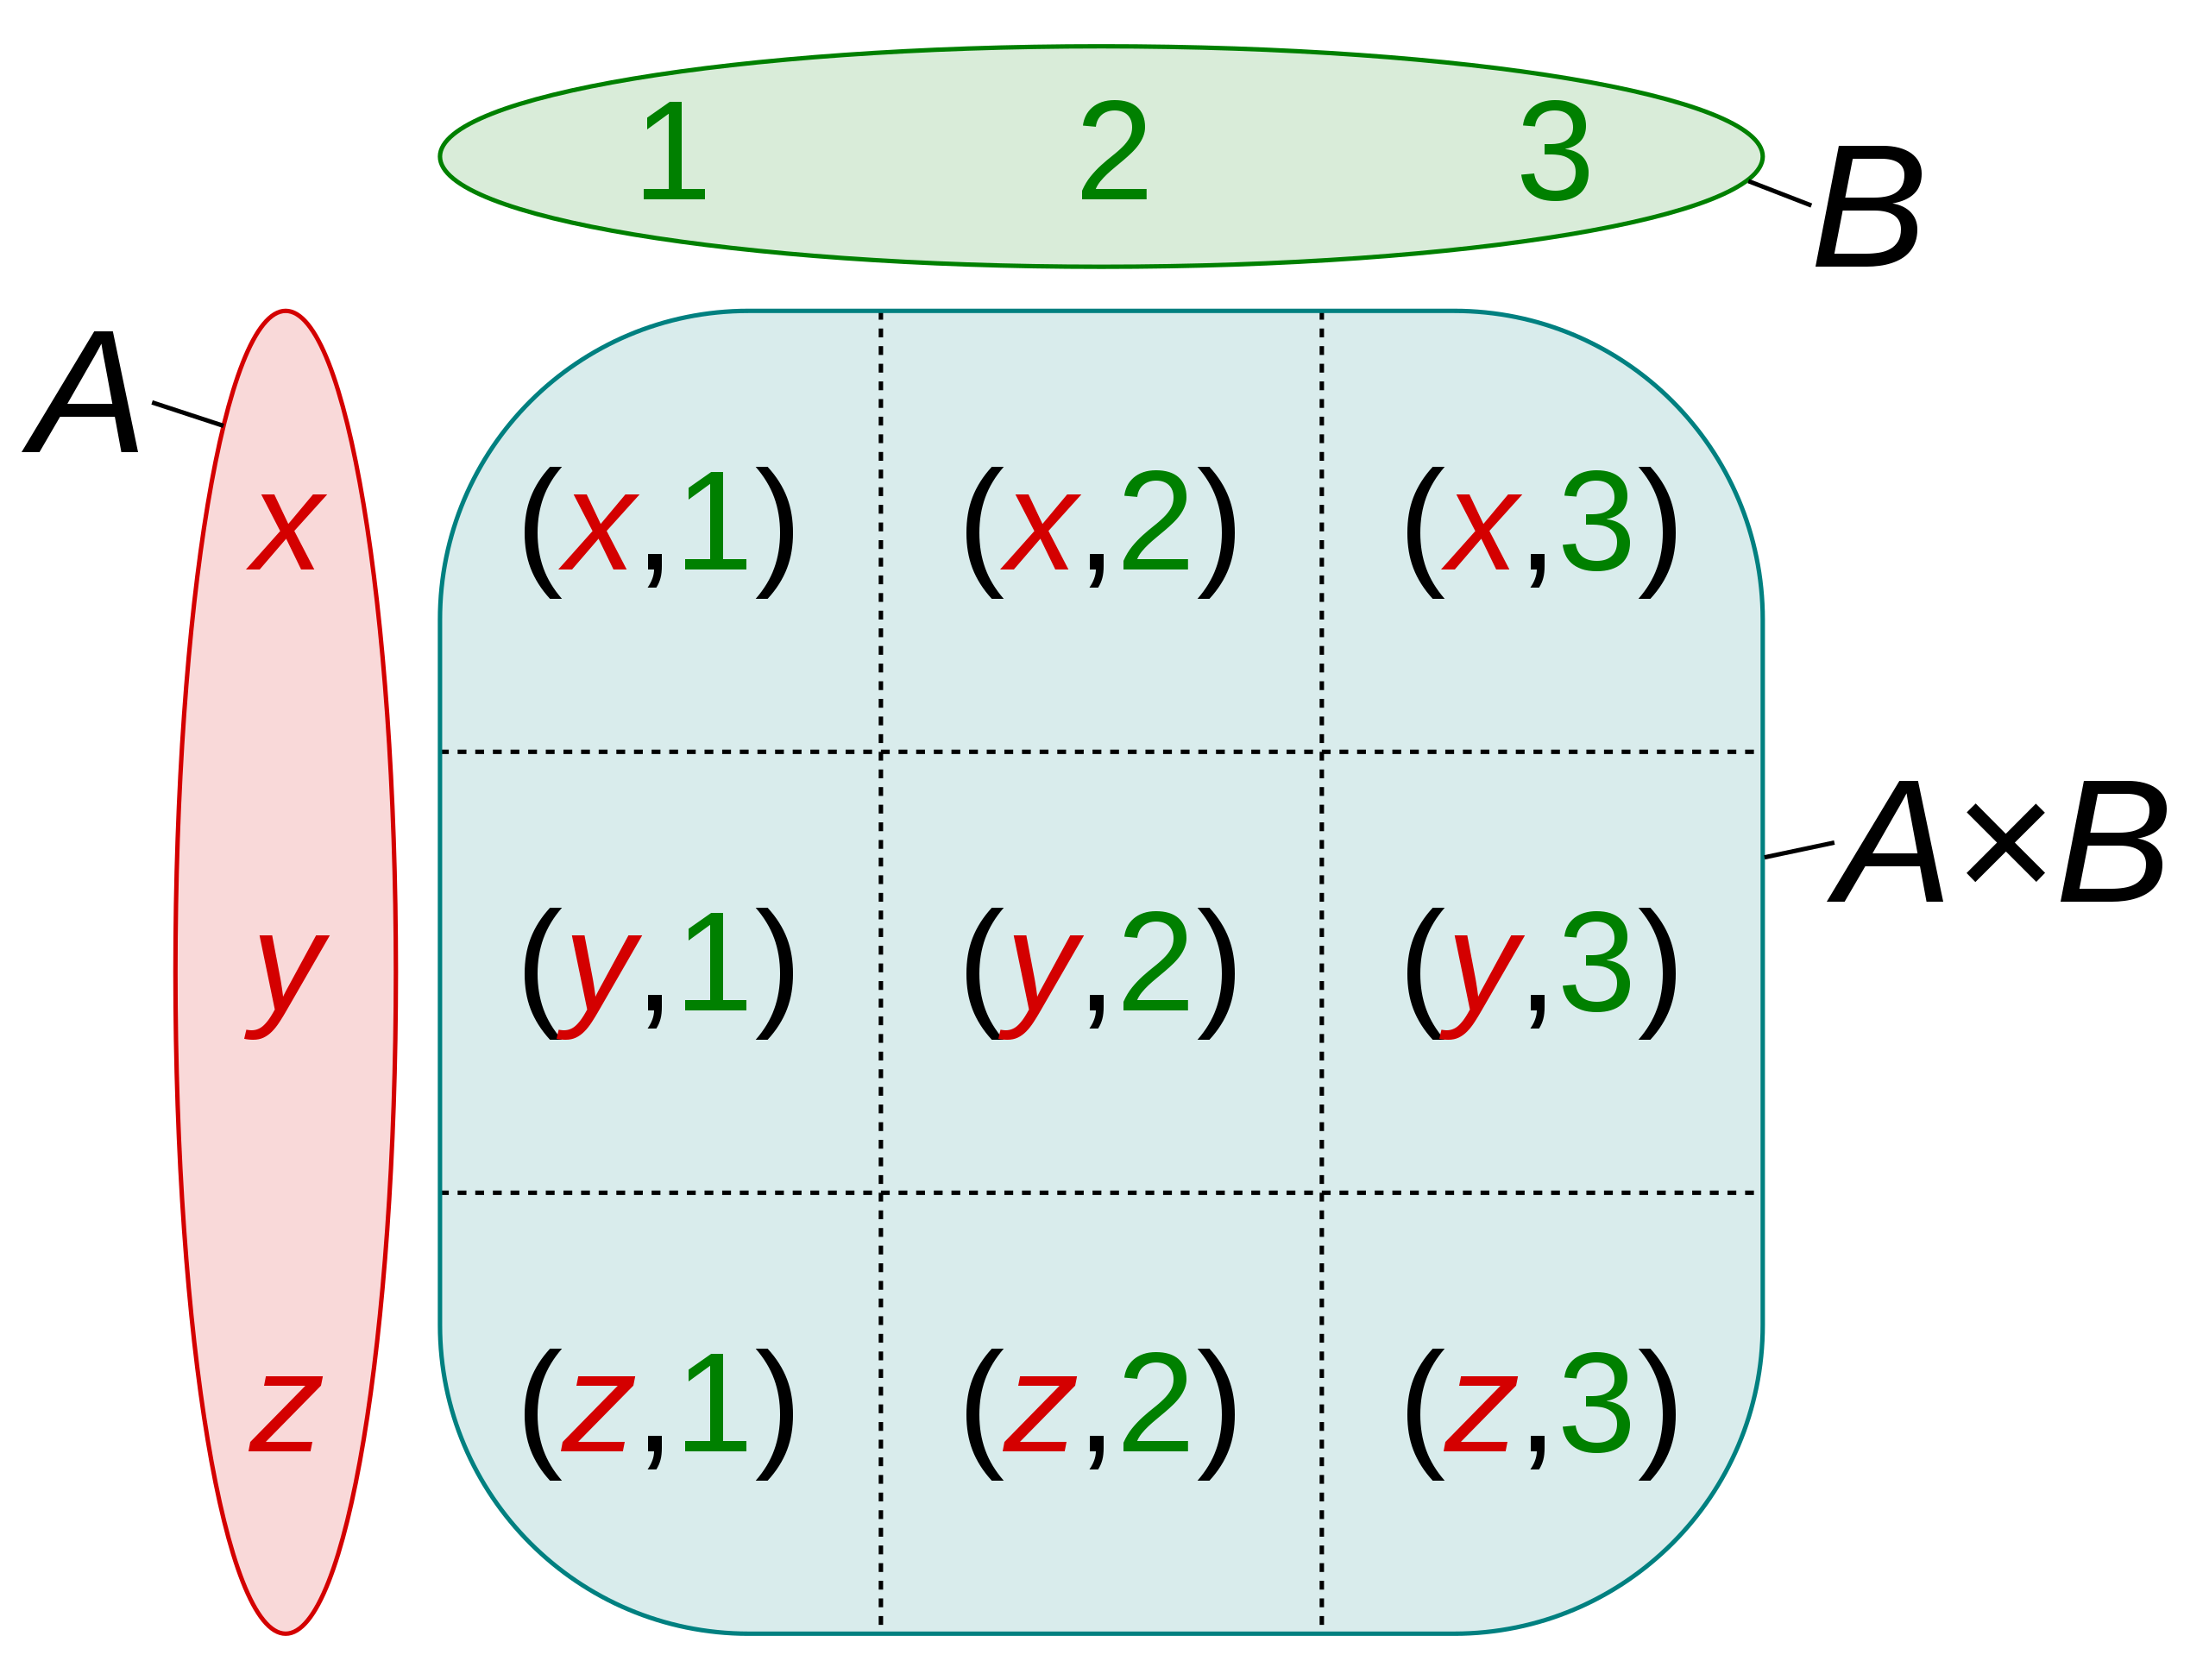
\includegraphics[scale=0.05]{Produit_Cartesien.png}
    \caption{Produit Cartésien(图源wiki)}
    \label{myref:Produit_Cartesien}
  \end{figure}
  \subsubsection{Exemple}
  我们最熟悉的平面直角坐标系就是$\R^2$.
  \subsection{De Morgan定律的集合形式}
  在集合论中,De Morgan定律表现为如下形式:
  \begin{itemize}
    \item $(A\cap B)^C=A^C\cup B^C $
    \item $(A\cup B)^C=A^C\cap B^C $
  \end{itemize}


  在经典命题逻辑的外延中,此二元性依然有效.即对于任意的逻辑运算符,我们都能找他它的对偶.
  这导致了基于传统逻辑的逻辑学的一个重要性质,即否定范式的存在性:如果其中否定仅出现在作用于公式中非逻辑的原子,任何公式都有它的等价公式.

  \section{公理化的集合论}\label{myref:gonglihua}
  主观意义上说,无论是ZF还是ZFC,在本讲义(或学院的课程)的“使用体验”上与原来朴素的直观的集合论没有什么区别,并且,有很多概念我们没有清晰.
  因此其实不必看懂这一章讲了什么,它不会影响你对后续章节内容的理解.
  \subsection{Russell悖论}
  现在,回头看看\prettyref{myref:quedingxing},尝试回答以下问题:\\
  设集合$A$是所有不属于自身的集合的集合,即$A=\{x | x\notin x\}$.那么请问$A$是否属于它自己?
  \begin{itemize}
    \item $A\in A$,说明$A$满足不满足其定义的不属于自身的性质,则$A\notin A$.
    \item $A\notin A$,说明$A$满足不属于自身的性质,则$A\in A$.
  \end{itemize}


  该悖论由数学家Bertrand Arthur William Russell提出,故称为Russell悖论.从经典逻辑的爆炸原理来看,任何命题都可以从矛盾中得到证明.
  因此,存在像Russell悖论这样的矛盾是灾难性的,因为如果任何公式可以被证明为真,它就破坏了真和假的含义.
  此外,由于集合论被视为所有其他数学分支公理化发展的基础,Russell悖论威胁到了整个数学的基础
  \footnote{
    其实除了Russell悖论,还有Burali-Forti悖论和Cantor悖论,但是相关的前置内容没有涉及,所以不放在这里讨论.
  },这激发了发展无矛盾的集合论的大量研究.
  \subsection{Zermelo-Fraenkel集合论:ZF公理体系}
  Zermelo-Fraenkel公理是众多集合论公理中的一员,也是对于不需要深入学习数学(特别是集合论)的我们最常见的公理体系.
  这套公理是二十世纪早期为了建构一个不会导致类似Russell悖论的矛盾的集合理论所提出的一个公理系统,简称为ZF公理.
  该公理体系包含以下公理:

    \subsubsection{外延性公理 Axiome d'extensionnalité}
      如果两个集合具有相同的元素则它们相等.\\\indent
      Si deux ensembles ont les mêmes éléments, alors ils sont égaux.
      $$
        \forall A\forall B,\forall x,(x\in A\Leftrightarrow x\in B)\Rightarrow A=B 
      $$

      \subsubsection{正规公理 Axiome de fondation/régularité}
      每个非空集合$X$都包含一个元素$y$,使得$X$和$y$不相交.\\\indent
      Tout ensemble $X$ non vide contient un élément $y$ tel que $X$ et $y$ sont des ensembles disjoints (qui n'ont aucun élément en commun).
      $$
        \forall X\neq \varnothing ,\exists y\in X,y\cap X=\varnothing 
      $$

      \subsubsection{分类公理 Schéma d'axiomes de compréhension/séparation}
      设$\mathbb{A}$为一个集合,且$P$为任一个描述$\mathbb{A}$内元素$x$的特征的性质,则存在$\mathbb{A}$的子集$A$包含$\mathbb{A}$内满足这个性质的$x$.\\\indent
      Pour tout ensemble $A$ et toute propriété $P$ exprimée dans le langage, il existe un ensemble dont les éléments sont les éléments de $A$ vérifiant $P$.
      $$
      \forall \{x| P(x) \}\subseteq \mathbb{A},\exists A\subseteq \mathbb{A},A=\{x| P(x)\}
      $$
      这样我们就可以定义空集了,例如对于集合$\mathbb{A},\varnothing =\{x|x\in\mathbb{Z}, x\neq x\}$.
      有时这也被称为空集公理(Axiome de l'ensemble vide).


      \subsubsection{配对公理 Axiome de la paire}
      若$X$和$Y$是集合,则存在一个集合包含$X$和$Y$. \\\indent
      Si $X$ et $Y$ sont deux ensembles, alors il existe un ensemble contenant $X$ et $Y$ et eux seuls comme éléments.
      $$
      \forall X\forall Y, \exists Z,X\in Z,y\in Z 
      $$

      \subsubsection{并集公理 Axiome de la réunion}
      对任一个集合$\mathcal{F}$,存在一个集合$A$,包含每个为$\mathcal{F}$的某个元素的元素的集合.\\\indent
      Pour tout ensemble $\mathcal{F}$, il existe un ensemble $A$ dont les éléments sont précisément les éléments des éléments de $\mathcal{F}$ et eux seuls.
      $$
      \forall \mathcal{F}\exists A,\forall F\subseteq\mathcal{F},\forall x\in F\Rightarrow x\in A 
      $$


      \subsubsection{替换公理 Schéma d'axiomes de remplacement}
      任何可定义函数下的集合的像也将落在集合内.\\\indent
      Pour tout ensemble $A$ et toute relation fonctionnelle $P$,formellement définie comme une proposition$P(x,y)$ et tel que $P(x,y)$ et $P(x,z)$ 
      impliquent que $y=z$, il existe un ensemble contenant précisément les images par $P$ des éléments de l'ensemble d'origine $A$.


      \subsubsection{无穷公理 Axiome de l'infini}
      存在包含无限多个元素的集合.\\\indent
      Il existe un ensemble $W$ dont $\varnothing$ est élément et tel que pour tout $X$ appartenant à $W$,$X\cup\{X\}$appartient aussi à $W$.
      $$
      \forall X,\, \exists \mathbb{W}, X\subseteq \mathbb{W}\Rightarrow X\cup \{X\}\subseteq \mathbb{W}
      $$


      \subsubsection{幂集公理 Axiome de l'ensemble des parties}
      对任一个集合$X$,存在一个集合$Y$为$X$的幂集的超集.\\\indent
      Pour tout ensemble $X$, il existe un ensemble dont les éléments sont précisément tous les sous-ensembles de $X$.
      $$
      \forall \mathbb{X},\exists \mathbb{Y},\forall X, X\subseteq \mathbb{X}\Rightarrow X\in\mathbb{Y}
      $$


      \subsubsection{良序定理 Théorème de Zermelo/du bon ordre}
      所有集合都可以被良序排序.\footnote{若给定前八个公理,就可以找到许多个和良序定理等价的叙述,例如选择公理.}\\\indent
      Tout ensemble peut être muni d'une structure de bon ordre.



  \subsection{选择公理 l'Axiome du choix: ZFC公理体系}
  对于所有的非空的索引族$(S_i)_{i\in I}$,存在一个索引集$(X_i)_{i\in I}$使得$\forall i\in I,X_i\in S_i $.
  它可以被理解为:给定任何非空集合的族,可以通过从每个集合中任意选择一个元素来构造一个新集合,即使其包含集合是无限的.\\

  对于Zermelo-Fraenkel集合论,若讨论的是其不包含学选择公理的形式,则称为ZF公理体系;若是其包含学选择公理的形式,则称为ZFC公理体系.
  


\chapter{映射\\ Applications}%同样这一张可以删除,或者放到前面去
内容调整中.
  \begin{figure}[H]
    \centering
    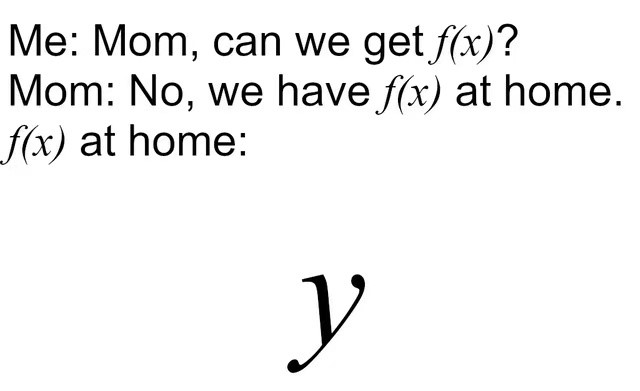
\includegraphics[scale=0.5]{yathome.jpg}
  \end{figure}


\chapter{运算与代数结构\\ Opérations et Structure Algébrique}
  
  \section{运算}
  在我的数学学习经历中,我最先认识了数字,也就是1、2、3、4这些,随后就开始学习了加法,然后是减法、乘法、除法之类的东西.
  这些东西都被称为运算.有些运算是一元的,例如$\cos x$和$|x|$,我们输入一个变量,得到一个返回结果;有些运算是二元(多元)的,例如$a^b$或者$A \times B$.本章里我们主要讨论二元运算.
  有些运算与数没有关系,例如逻辑运算里,$1\vee 0=1$,这里1和0只是表示逻辑上的真和假,与具体的数字无关.
  此外,还有一种题目叫做“定义新运算”,一般会给出一个自定义的算符,比如$\star $,然后解释这个算符怎么计算,比如说$a\star b=114a+\frac{514}{b}-19^{\frac{a}{b}}$,让你求解一些具体的返回值.
  这些统统都是运算.为了应付日益复杂的数学,我们需要把运算统一起来研究,以便于尝试找到普适性的规律.\label{myref:traditionalcalculate}
  \subsection{Définition}
  给定集合$X$,所有$f:X\times X\rightarrow X$的映射称为集合$X$上的运算.直观上看,运算将$X$上的有序点对映射为$X$的元素.
  我们姑且将运算符号记为$\star $.
  这样我们可以将一个运算表示为$(x,y)\in X*2,f(x,y)\rightarrow x\star y$.
  \subsubsection{Exemple}
  在$\R$上两个区间的并$(-114,81]\cup (-91,514)=(-114,514)$是一个运算.
  \subsection{结合律 Associative}
  设$X$上的运算$f(x,y)\rightarrow x\star y $,若:
  $$
  \forall (x,y,z)\in X^3, x\star(y\star z)=(x\star y)\star z
  $$
  称此运算满足结合律.
  \subsection{交换律 Commutative}
  设$X$上的运算$f(x,y)\rightarrow x\star y $,若:
  $$
  \forall (x,y)\in X^2, x\star y=y\star x
  $$
  称此运算满足交换律.
  \subsection{中性元/单位元 l'élément neutre/identité}
  单位元又叫中性元.设$X$上的运算$f(x,y)\rightarrow x\star y $,若:
  $$
  \forall x\in X, \exists e\in X,e\star x=x
  $$
  称$e$是左单位元,若:
  $$
  \forall x\in X, \exists e\in X,x\star e=x
  $$
  称$e$是右单位元,若$e$同时为左单位元及右单位元,则称$e$为单位元.
  单位元也被记作$\Id$,即identité的前两个字母.或者在很多地方都有自己的记号.
  \subsubsection{Exemple}
  $\R $上的加法单位元为0,乘法单位元为1.幂运算$a\star b=a^b$的右单位元为1,没有左单位元.
  \subsubsection{Exemple}
  集合$X$上交集运算的单位元为$X$,并集运算的单位元为$\varnothing $.
  \subsubsection{Exemple}
  设集合$A=\{e,f\}$上的运算为:
  $$
    \begin{aligned}&
    e\star e=f\star e=e\\&
    f\star f=e\star f=f
  \end{aligned}
  $$则$e,f$都是左单位元.
  \subsubsection{Proposition:单位元唯一}
  一个运算如果有单位元,则单位元是唯一的.
  \subsubsection{Démonstration}
  $\lnot (\text{单位元是唯一的})\Rightarrow \exists (e_1,e_2)\text{都是单位元}\Rightarrow e_1\star e_2=e_1,e_1\star e_2=e_2\Rightarrow e_1=e_2$
  \subsubsection{Remarque}
  一个运算有若干个左单位元是可能的.
  事实上,每一个元素都可以是左单位元.同样地,右单位元也一样.
  但若同时存在有右单位元和左单位元,则它们会相同且只存在一个单位元.
  
  \subsection{可逆元/可对称元 Symétrique}
  设$X$上的运算$f(x,y)\rightarrow x\star y $有单位元$e$,若:
  $$
  \forall x\in X, \exists x'\in X,x'\star x=e
  $$
  称$x'$是左可对称的,若:
  $$
  \forall x\in X, \exists x'\in X,x\star x'=e
  $$
  称$e$是右可对称的.所有满足$x\star x'=x'\star x=e$的$x'$称为$x$的可对称元.使用乘法符号时一般把可对称称为可逆,$x'$记作$x^{-1}$.
  
  \section{符合结合律的有单位元运算}
  符合结合律且有单位元的运算具有一些有趣的性质.本节讨论均假设$X$上满足结合律的运算$f(x,y)\rightarrow x\star y $有单位元$e$.
  \subsection{可对称元唯一性}
  当且仅当左对称元$x'$和右对称元$x''$是唯一且相同时,$x$是可对称的.
  \subsubsection{Démonstration}
  $$
    x''=e\star x''=(x'\star x)\star x''=x'\star(x\star x'')=x'\star e=x'
  $$
  \subsection{可对称的运算不变性}
  若$x$和$y$是可对称的,则$x\star y$也可对称,且$(x\star y)'=y'\star x'$.
  \subsubsection{Démonstration}
  $$
    (y'\star x')\star(x\star y)=y'\star (x'\star x)\star y=y'\star e\star y=y'\star y=e
  $$反过来同理.
  \subsection{解的唯一性}
  设$a$可对称,对于$b$,仅有唯一一个$x$使得$a\star x=b$,即$x=a'\star b$.
  \subsubsection{Démonstration}
  $$
    a\star x=b\Rightarrow a'\star b=a'\star (x\star x)=(a'\star x)\star x=e\star x=x
  $$反过来同理.
  这意味着,例如,在乘法中,形如$ax=b$的方程有且仅有唯一解$x=a^{-1}b$.

\section{代数结构 Structure Algébrique}
  在数学中,代数结构由非空集合$A$和$A$上的运算集合(通常是二元运算)和一组有限的恒等式(公理)组成,这些运算必须满足这些公理.
  研究代数结构的好处在于,当一个新问题涉及与这种代数结构相同的定律时,仅使用结构定律证明的所有结果都可以直接应用于新问题.
  \subsubsection{Exemple}
  $\R$上的加法$(\R,+)$就是一个代数结构,其具有以下公理:
  \begin{itemize}
    \item 交换律:$a+b=b+a$.
    \item 结合律:$(a+b)+c=a+(b+c)$.
    \item 单位元0:  $a+0=0+a=a$.
    \item 可逆性:$a+(-a)=(-a)+a=0$.
  \end{itemize}
  \subsubsection{Exemple}
  回看前言里\prettyref{myref:abstract}所展现的分析学知识,可见大部分内容都与代数结构相关.
  \subsection{封闭性}
  当我们想使用一个代数结构,也就是对一个集合上的元素进行运算时,为了得到一些良好的性质或者进行后续的运算,
  我们通常希望运算的结果能拥有一些性质.最简单的就是这个结果可以再次被拿来运算.这意味着这个运算结果也属于代数结构的集合.
  也即$$\forall (x,y)\in A\times A, x\star y=z \Rightarrow z\in A$$这样的性质称为封闭性.


  想象一个没有封闭性的代数结构上的运算,比如$\R$上,某个运算结果为:$1\star 4=\text{西红柿炒鸡蛋}$.
  显然,1和4都在$\R$上,但是西红柿炒鸡蛋不属于$\R$,我们也并不清楚西红柿炒鸡蛋有什么性质,它与$\R$上的元素有什么关系,也不能拿来继续运算.这样的性质就很糟糕.\\
  
  现在,我希望你假装忘记掉曾经学习的这些运算,也就是\prettyref{myref:traditionalcalculate}开头我提到的那些以前的东西(特别是加法和乘法),以便我们从另一个角度重新出发学习它们.

\section{群 Groupe}
  \subsection{Définition}
  群是一种代数结构,依托于集合上的运算"$\times$",称为"乘法",记为$(G,\times)$或者$(G,\cdot)$(有时运算符号可省略).
  为了避免与笛卡尔积混淆,我们统一采用$(G,\cdot)$记号.
  其满足以下公理:
  \begin{itemize}
    \item 封闭性:$\forall(a,b)\in G^2,a\cdot b=c\in G $.
    \item 结合律:$\forall(a,b,c)\in G^3,(a\cdot b)\cdot c=a\cdot (b\cdot c) $.
    \item 单位元e: $\forall a\in G, \exists e\in G, a\cdot e=e\cdot a=a$.
    \item 可逆性:  $\forall a\in G, \exists a^{-1}\in G, a\cdot a^{-1}=a^{-1}\cdot a=e$.
    \item \textbf{Bonus:}交换律:$\forall(a,b)\in G^2,a\cdot b=b\cdot a $.
  \end{itemize}
  满足前四项公理的代数结构称为群.额外满足第五项交换律的群称为"阿贝尔群(Groupe Abélien)".
  \subsubsection{Exemple}
  \begin{itemize}
    \item 整数的通常意义加法$(\mathbb{Z},+) $构成群,但是通常意义乘法$(\mathbb{Z},\cdot) $不构成群,因为不满足有可逆元.
    \item (n阶非奇异矩阵\footnote{万一你还没学过这个定义,它意味着矩阵的行列式值不等于0.},矩阵乘法)是一个群.



  \end{itemize}
  \subsection{阶 Ordre}
  在有限群范围内,群$(G,\cdot)$的阶等于集合$G$里元素的个数,也就是$|G|=\text{card }G$.
  元素的阶等于让该元素通过幂运算得到单位元的最小幂,也就是$n_{min},a^n=e$.

  \subsection{乘法表 Table de multiplication}
  乘法表常被用来表示简单的群上的元素和运算,它列举了群内任意两个元素的乘积.下面我们通过一个简单的例子来理解乘法表.
  \subsubsection{$C_3$群}\label{myref:C_3}
  想象一个等边三角形$\Delta ABC$,我们将它绕着垂直于几何中心的州进行旋转操作:
  \begin{itemize}
    \item 操作a:顺时针旋转120°
    \item 操作b:逆时针旋转120°
    \item 操作e:不旋转
  \end{itemize}
  我们发现,经过操作a后,原来的A点变成了B点,B点变成了C点,C点变成了A点,得到了三角形$\Delta BCA$.
  而与此同时,经过两次操作b后也能让原来的A点变成了B点,B点变成了C点,C点变成了A点.也就是说,两次操作b与一次操作a等价.同理,两次操作a与一次操作b等价.
  进一步地,我们发现,三次操作a、三次操作b、操作b后操作a、操作a后操作b与操作e相互都是等价的.如果我们把操作看作一个集合,操作的复合看作运算$\cdot $,就得到了一个群.其中的运算关系如下:
    \begin{itemize}
    \item $a=b\cdot b=a\cdot e$
    \item $b=a\cdot a=b\cdot e$
    \item $e=e\cdot e=a\cdot a\cdot a=b\cdot b\cdot b=a\cdot b=b\cdot a$
    \end{itemize}
  这个群被称为$C_3$群.其阶数为3,元素a和b的阶数也是3.
  将这些运算关系组合成一个表,第一行表示在运算符号前的元素,第一列表示运算符号后的元素,就可以填入所有的运算结果.也即:
  \begin{table}[!h]
    \centering
    \begin{tabular}{r|lll}
         ($C_3,\cdot$) & \textbf{a} & \textbf{b} & \textbf{e} \\ \hline
        \textbf{a} & b & e & a \\ 
        \textbf{b} & e & a & b \\ 
        \textbf{e} & a & b & e \\ 
    \end{tabular}
    \caption{$C_3$群的乘法表}
    \label{C_3times}
  \end{table}
  \subsection{重排定理 Théorème de réarrangement}
  考虑代数结构$(A,\star)$,对$a\in A$,定义$a\star A=\{ a\star a_\alpha|a_\alpha \in A \}$.对群$G$,有:
  $$
  \forall a\in G,a\cdot G=G\cdot a=G
  $$也即群内的每个元素和某个元素相乘得到的仍然是原来的群,这被称为群的重排定理.
  \subsubsection{Démonstration}
  由运算的封闭性知$a\cdot G\subseteq G$,
  由可逆性知$\forall (a,g)\in G\times G, \exists (a'\cdot g)\in G\text{使得}g=a\cdot (a'\cdot g)=g\Rightarrow g\in a\cdot G\Rightarrow G\subseteq a\cdot G$.
  \subsection{生成元 Générateur}
  生成元是描述一个群的重要方式.下面我们由循环群开始逐渐介绍生成元和其应用方法.
  \subsubsection{循环群 Groupe cyclique}
  由一个元素$R$及其幂次构成的有限群称为由$R$生成的循环群,记为$C_n$,其中\n 为循环群的阶,$R$称为循环群的生成元.
  这就是为什么\prettyref{myref:C_3}介绍的群叫$C_3$群.在$C_3$群中,a和b都是其生成元.对于\n 阶循环群, 其阶数等于其生成元的阶数.
  \subsubsection{有限群的生成元与秩 Générateur et rang d'un groupe fini}
  对任一有限群, 是否同样有生成元呢?答案是肯定的,由此还能引出有限群的秩的概念.对有限群$G$,任取一元素$R_1$,得到其幂次构成的集合$\mathbf{R_1}$.
  若$\mathbf{R_1}^C\neq \varnothing$,即无法填满整个群,则在$\mathbf{R_1}^C$内任取一元素$R_2$并得到$\mathbf{R_2}$,以此类推.
  将选取的元素组成集合$\{R_i\}$,该集合即为群$G$的生成元,且$\text{card}\{R_i\}$称为群的秩.
  \subsubsection{Proposition}
  有限群的生成元的选择不唯一,但秩不变.

  \section{从原群到群 De magma à groupe}
  一个代数结构想成为群需要符合四个条件,那不能全部符合四个条件的代数结构又是什么呢?
  \subsection{原群 Magma}
  对代数结构$(E,\star)$,若其运算满足封闭性,则该代数结构为一个原群.

  \subsection{半群 Demi-groupe}
  对原群$(E,\star)$,若其运算满足结合律,则该原群为一个半群.

  \subsection{幺半群 Monoïde}
  对半群$(E,\star)$,若其含有中性元,则该半群为一个幺半群.

  \subsection{拟群 Quasigroupe}
  对原群$(E,\star)$,若有:
  $$
  \forall (a,b)\in E\times E, \exists (x,y)\in E\times E\text{使得}a\star x=y\star a=b
  $$则该原群为一个拟群.


  \begin{figure}[H]
    \centering
    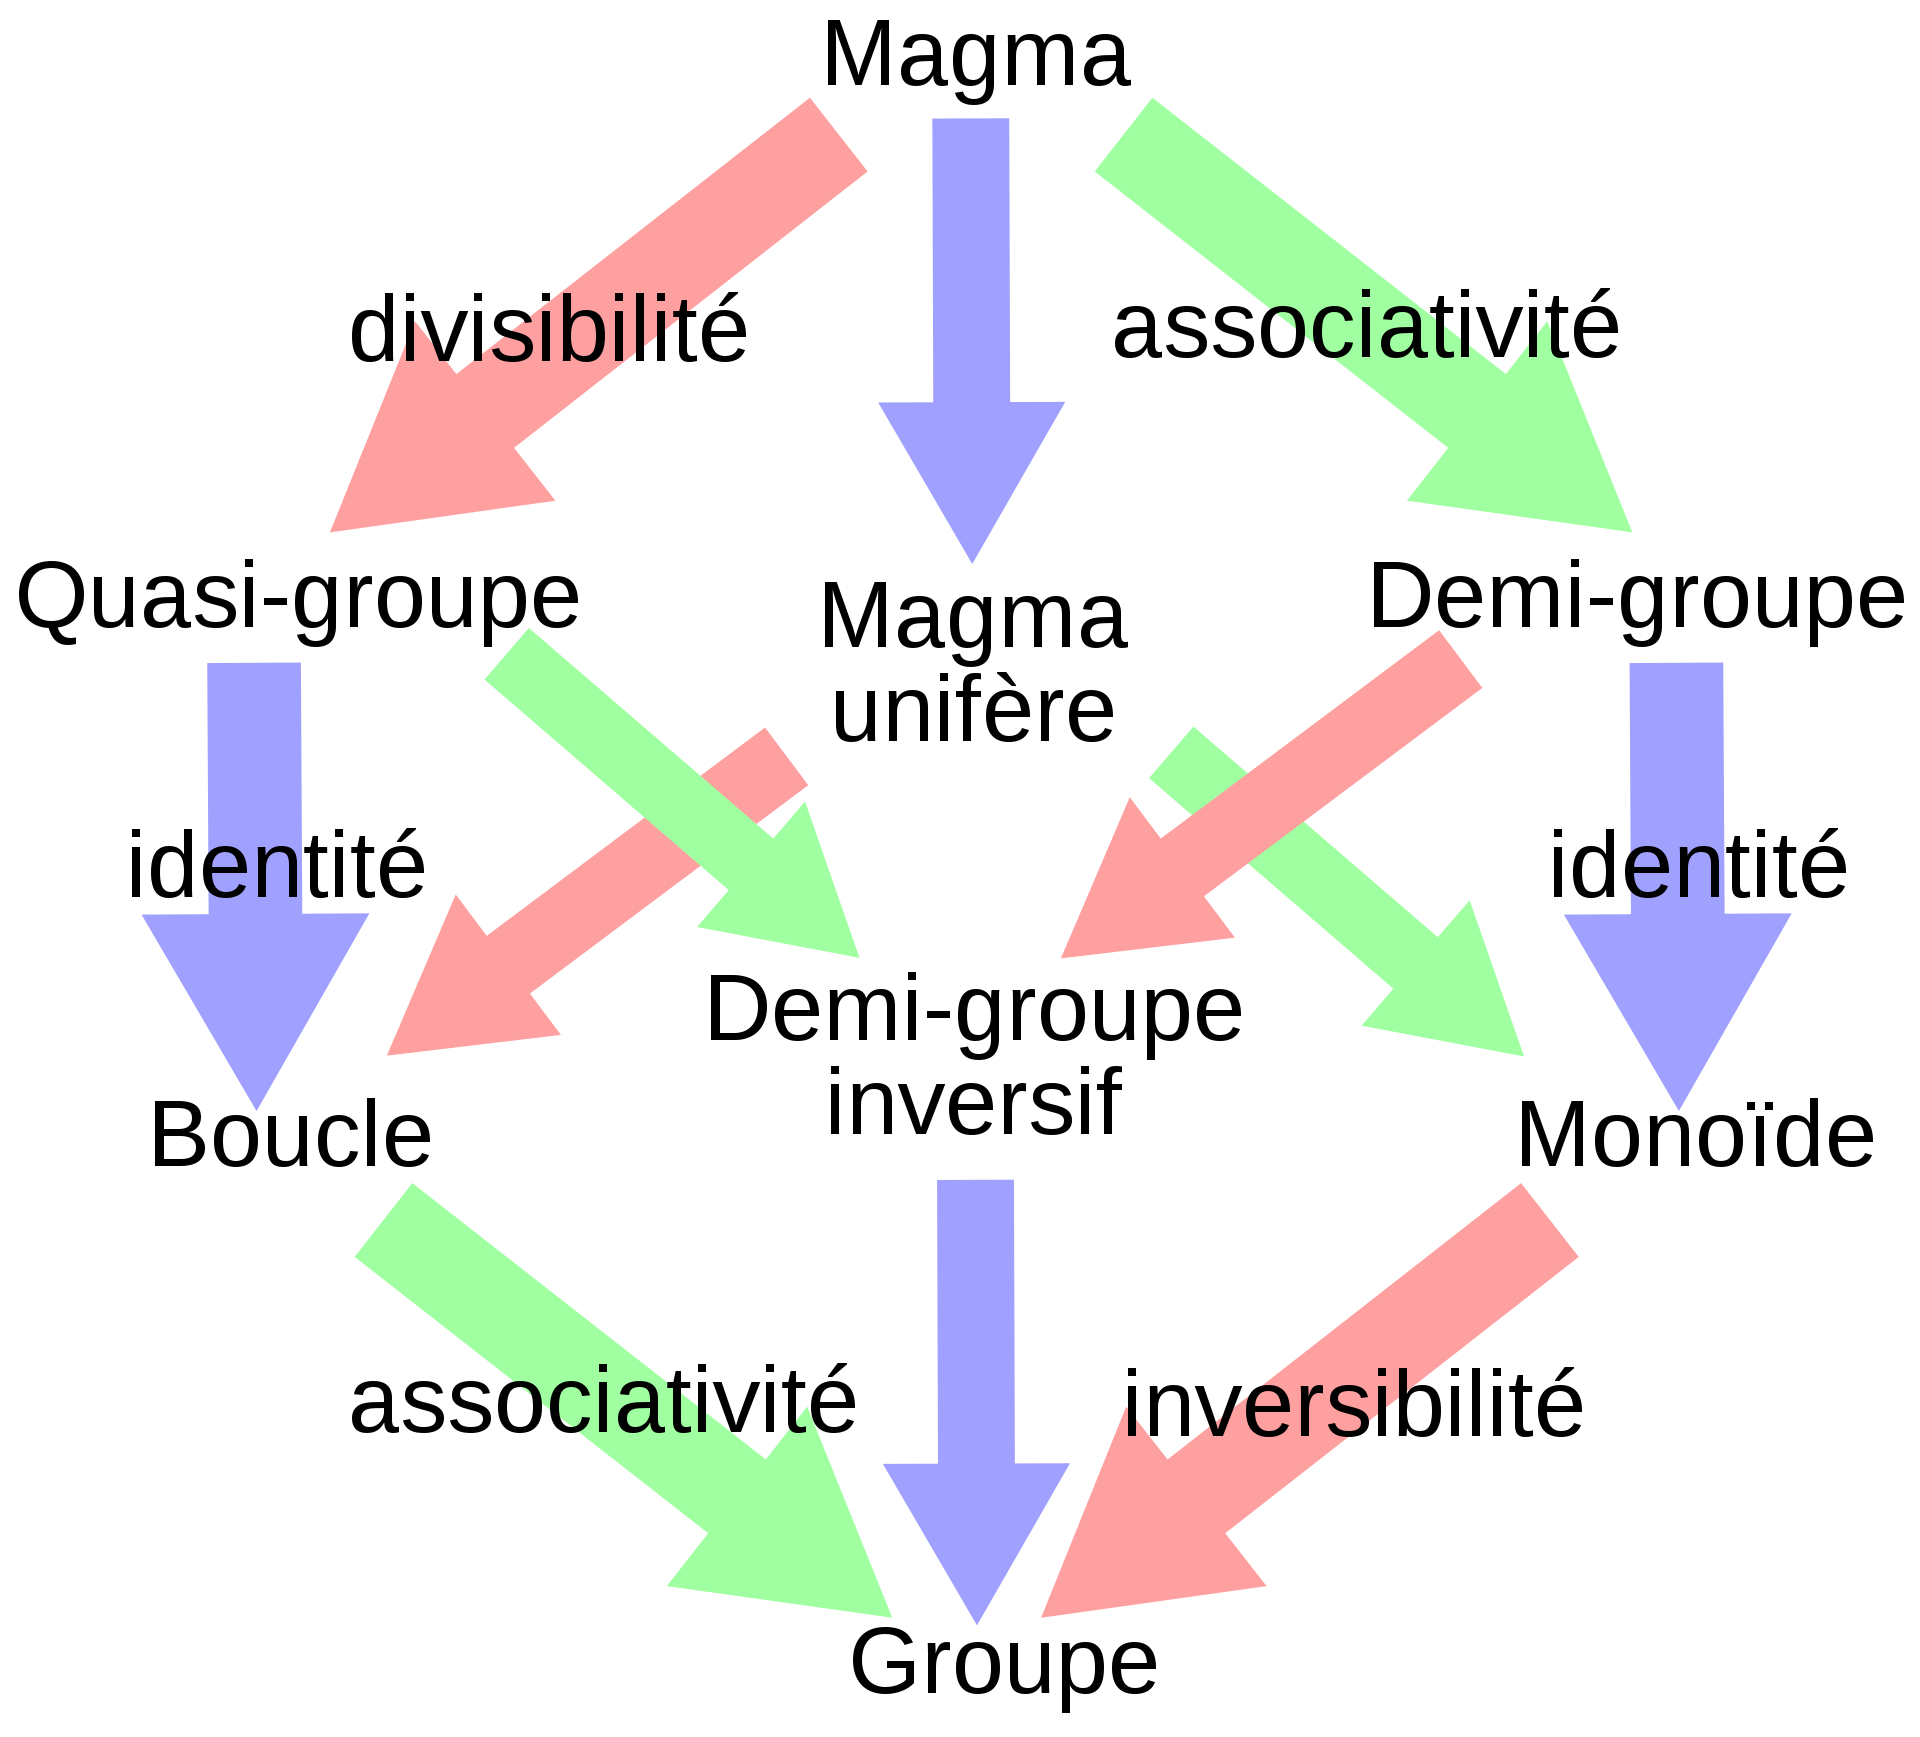
\includegraphics[scale=0.13]{magma_groupe.png}
    \caption{从原群到群(图源wiki)}
    \label{myref:groupe_magma}
  \end{figure}

  \section{群论基础 La Théorie Rudimentaire des Groupes}
  在数学中,特别是在一般代数中,群论是研究群的代数结构的学科.群论的发展起源于数论、代数方程理论和几何学,在理论物理、化学、材料科学和非对称密码学中有多种应用.
  本章只对群论内容做一个基础的、入门的介绍.事实上,关于群、环和域相关的知识在本讲义中并不怎么重要,很多结论也不会有后续应用(所以有相当多平凡的推论我没有写出证明,摸了).但是有些概念和定义还是会用上的,因此我还是简单地列出来.

  \subsection{共轭关系 Conjugaison}\label{myref:conjugaison}
  定义二元关系~为:对$(a,b)\in G\times G, \exists g\in G$使得$b=g^{-1}\cdot a\cdot g$.称该关系为共轭关系,a~b为a与b共轭.
  \subsubsection{Proposition}
  共轭关系是等价关系.
  \subsubsection{Démonstration}
  \begin{itemize}
    \item $a=a^{-1}\cdot a\cdot a\Rightarrow a\sim a$
    \item $a\sim b\Rightarrow b=g^{-1}\cdot a\cdot g\Rightarrow g\cdot b\cdot g^{-1}=a\Rightarrow a=(g^{-1})^{-1}\cdot b\cdot g^{-1}\Rightarrow b\sim a$
    \item $b=g^{-1}\cdot a\cdot g, c=f^{-1}\cdot a\cdot f\Rightarrow b=f\cdot c\cdot f^{-1}=g^{-1}\cdot a\cdot g\Rightarrow c=(f^{-1}\cdot g^{-1})\cdot a\cdot (g\cdot f)\Rightarrow c\sim a$
  \end{itemize}
  \subsubsection{共轭类 Action par conjugaison}
  a的共轭类是群内所有与其共轭的元素组成的集合,记为$Cl(a)$或$C_a$,即$Cl(a)=\{g\cdot a\cdot g^{-1}|g\in G\}$.\\

  接下来给出一些共轭类的简单推论:
  \subsubsection{Proposition}
  $a\sim b\Leftrightarrow Cl(a)\cap Cl(b)\neq \varnothing$
  \subsubsection{Proposition}
  共轭类内元素的阶相同.
  \subsubsection{Proposition}
  单位元e只与自己共轭.
  \subsubsection{Proposition}
  Abel群里每个元素只与自己共轭.
  \subsubsection{Proposition}
  $a\sim b\Rightarrow \forall k\in \mathbb{N},a^k\sim b^k$.

  \subsection{子群 Sous-groupe}
  直观上说,子群就是群的一个同样是群的子集.
  \subsubsection{Définition}
  对群$(G,\cdot)$,若$H\subseteq G$使得$(H,\cdot)$也是一个群,则称$H$是$G$的子群.
  \subsubsection{Proposition}
  $G$和$\{e\}$显然都是子群.它们被称为平凡子群(sous-groupe trivial)或者 sous-groupe impropre.
  不是平凡子群的子群称为特征子群(sous-groupe propre).
  \subsubsection{Remarque}
  质数阶(或者1阶)循环群没有特征子群.
  \subsubsection{Proposition}
  对于$pq$阶循环群($p,q$为正整数),其只有一个$p$阶子群.该子群是由$g^q$生成的循环群.

  \subsection{陪集 Classe suivant un sous-groupe}
  法语里并没有专门的陪集的专有名词,而是直接叫classe suivant un sous-groupe,这是个很形象的说法.英语称陪集为coset,其实也和suivant有异曲同工之妙吧.
  \subsubsection{Définition}
  群$(G,\cdot)$有子群$H$.对任意$g\in G$,$H$有如下两个陪集:
  \begin{itemize}
    \item 左陪集(classe à gauche de $g$ suivant $H$): $gH=\{g\cdot h|h\in H\}$
    \item 右陪集(classe à gauche de $g$ suivant $H$): $Hg=\{h\cdot g|h\in H\}$
  \end{itemize}
  \subsubsection{陪集分解 Décomposition en classes suivant un sous-groupe}
  群$G$可以被分解成若干个左陪集的并,或者若干个右陪集的并.对应的分解称为左/右陪集分解.即:
  $$
  G=\bigcup_{\alpha\in G}\alpha H= \bigcup_{\alpha\in G}H\alpha
  $$
  \subsubsection{Proposition}
  $f\in gH\Leftrightarrow fH=gH,f\in Hg\Leftrightarrow Hf=Hg$.
  \subsubsection{Proposition}
  $gH=H\Leftrightarrow g\in H\Leftrightarrow Hg=H$.
  \subsubsection{Proposition}
  $|gH|=|H|$
  \subsubsection{Proposition}
  “属于同一左陪集”是一个等价关系.
  \subsubsection{Proposition}
  任意两个左陪集要么不相交要么相等.

  \subsection{群论的Lagrange定理 Théorème de Lagrange}
  Lagrange定理的直接叙述为:子群的阶整除群的阶,即:若群$(G,\cdot)$有子群$H$,则$|G|=k|H|,k\in\mathbb{N}$.
  将其倍数$k$记为$[G:H]$,表示$H$在$G$中左陪集的个数.
  \subsubsection{Démonstration}
  考虑子群$H$关于$G$内所有元素的左陪集组成的集族$\mathbb{H}=\{g_iH|g_i\in G\},\text{每个左陪集的阶都相同,}|g_jH|=|g_kH|$并且$\sum_{i}^{\text{card }\mathbb{H}}|g_iH|=|G|$
  此时$\text{card }\mathbb{H} $就是$[G:H]$.
  \subsubsection{Proposition}
  素数阶的群只有平凡子群,没有特征子群.
  \subsubsection{Proposition}
  元素的阶整除群的阶.(元素的阶可以组成子群)
  \subsubsection{Fermat小定理 Théorème de Fermat}
  对整数$a$和素数$p$,若$a$不是$p$的倍数,则$a^p-1$是$p$的倍数,即:
  $$
    a^{p-1}\equiv 1(\mod p)
  $$
  \subsubsection{Démonstration}
  为了证明这个推论,我们考虑$G=\{1,2,\dots , p-1\}$和模运算组成的群.假设$a\equiv b(\mod p),\text{显然}b\in G$.
  设$b$的阶数为$k$,即$b^k\equiv 1(\mod p)$,则可得到子群$H=\{a,b,\dots ,b^{k-1}\}$则$k$可以整除$G$的阶数,也就是$p-1$.
  此时再设$p-1=km$,此时有:
  $$
    a^{p-1}\equiv b^{km}\equiv (b^k)^m\equiv 1^m\equiv 1(\mod p)
  $$得证.
  \subsection{正规子群 Sous-groupe normal}
  正规子(Sous-groupe normal) 又叫不变子群(Sous-groupe invariant),法语里还有称Sous-groupe distingué.其代表共轭变换下不变的子群.
  \subsubsection{Définition}
  对群$(G,\cdot)$,若子群$N$满足:
  $$
  \forall n\in N,\forall g\in G,g\cdot n\cdot g^{-1}\in N
  $$则称$N$是$G$的正规子群,记作$N\lhd G$或者$N\unlhd G$.
  \subsubsection{等价条件}
  下列条件等价于子群N在G中是正规子群:
  \begin{itemize}
    \item $\forall g\in G,gNg^{-1}\subseteq N $
    \item $\forall g\in G,gN=Ng $
    \item $\forall (g,h)\in G\times G,gh\in N\Leftrightarrow hg\in N$
  \end{itemize}


  \subsection{商群 Groupe quotient}
  \subsubsection{子群的乘法}
  设群$(G,\cdot)\text{有子群}H\text{和}F$,定义其乘法为:
  $$
  H\cdot F=\{h\cdot f|(h,f)\in G\times F \}
  $$
  \subsubsection{Définition}
  利用正规子群的左陪集和右陪集相同的这个特点将群按照陪集的方法进行分割.
  分割后的所有陪集形成的集合能够形成一个新的群,称之为商群,记为$G/H$.也即:
  $$
  G/H=\{gH\text{ }|H\lhd G,g\in G \}
  $$
  \subsubsection{Démonstration}
  \begin{itemize}
    \item 单位元: $aH=H=Ha$
    \item 逆元: $aH\cdot a^{-1}H=aa^{-1}HH=H$
    \item 结合律: $aH\cdot bH\cdot cH=(ab)cH=a(bc)H=aH\cdot(bH\cdot cH) $
    \item 封闭性: $aH\cdot bH=(ab)H\in G/H $
  \end{itemize}
  \subsubsection{Proposition}
  $|G/H|=[G:H]$,商群的阶是群的阶除以子群的阶的商.
  \subsubsection{Proposition}
  若$(G,\cdot)$是Abel群/循环群/有限生成群,则$G/H$也是.

  \subsection{同态 Homomorphisme}    \label{myref:Homomorphisme}
  \subsubsection{Définition}
  同态是两个群之间的一种特殊的映射,其概念非常直观.“同”表示映射的两端有什么东西是一样的,或者不变的.“态”就是群的某种“状态”.
  群只有集合和运算两个要素,集合映射过去后不可能保持不变,那能保持的也就只有运算了.因此,同态就是两个群之间保持乘法运算的映射,即
  对于$(G,\cdot)$和$(H,\star)$上的映射$f:G\rightarrow H $,若
  $$
    \forall (x,y)\in G\times G,f(x\cdot y)=f(x)\star f(y)
  $$称$f$是$(G,\cdot)$和$(H,\star)$上的同态映射.存在同态映射的两个群是同态的.若同态是单射,则称单同态(Monomorphisme),若为满射则称满同态(Épimorphisme).
  \subsubsection{Exemple}
  正实数上通常加法群到通常乘法群上的映射$f(x)=e^x$就是一个同态.$e^{a+b}=e^a\cdot e^b$.
  \subsubsection{Proposition}
  同态的一个重要性质是保证了单位元映射到单位元,$f(e_G)=e_H$.
  \subsubsection{自同态 Endomorphisme}
  群$(G,\cdot)$到自身上的同态映射称为自同态.
  \subsubsection{态射 Morphisme}
  同态的推广被称为态射.在讨论群的内容时,法语有时直接用态射指代同态,记住两者在此时是同一概念.
  \subsection{同构 Isomorphisme}    \label{myref:Isomorphisme}
  若同态映射$f$为双射,则称为同构映射,两个群是同构的,记作$G\cong H$.
  \subsubsection{Proposition}
  同构是等价关系.

  \subsubsection{自同构 Automorphisme}
  同理,群$(G,\cdot)$到自身上的同构映射称为自同构.
  \subsubsection{Remarque: 同构与相等}
  一般来说,如果忽略掉同构的对象的属性或操作的具体定义,单从结构上讲,同构的对象是完全等价的.
  但这并不意味着同构就是相等.例如,我们很容易知道$C_3$群可以和某个群\{西红柿炒鸡蛋,醋溜土豆丝,糖醋排骨\}同构(例如
  $f(a)=\text{西红柿炒鸡蛋},f(b)=\text{醋溜土豆丝},f(e)=\text{糖醋排骨}$),
  但这并不代表两个群,或者两个集合就是相等的.起码西红柿炒鸡蛋不在$C_3$群里面.

  \subsection{核 Noyau}
  \subsubsection{Définition}
  对于同态$f:G\rightarrow H $, $G$中映射到$H$单位元的元素称为同态的核,记作:
  $$
  \ker f=\{f(g)=e_H\text{ }|\text{ }g\in G  \}
  $$
  \subsubsection{Proposition}
  $\ker f\lhd G$,核是正规子群.
  \subsubsection{Proposition}
  $G/\ker f\cong H$,核的商群与$H$同构.\\
  
  其实到这里我想接着讲同构基本定理的,
  但是这一章内容太多了,而且毕竟不是写代数讲义,因此我们点到为止,快速过完这一章的内容.


  \section{环 Anneau}
  \subsection{Définition}
  与群类似,环也是一种代数结构,依托于集合上的运算“$+$”和“$\times$”,分别被称为“加法”和“乘法”.同样将乘法符号记为$\cdot$,
  则一个环写作$(R,+,\cdot)$.其满足以下公理:\\

  \noindent
  1.$(R,+)$是Abel群,即:
  \begin{itemize}
    \item 封闭性:$\forall(a,b)\in R^2,a+b=c\in R $.
    \item 结合律:$\forall(a,b,c)\in R^3,(a+ b)+ c=a+ (b+ c) $.
    \item 单位元0: $\forall a\in R, \exists 0\in R, a+0=0+a=a$.
    \item 可逆性: $\forall a\in R, \exists -a\in R, a+(-a)=(-a)+a=0$.有时将此类运算用减法符号代替,即$a+(-b)=a-b$,这样就熟悉多了.
    \item 交换律:$\forall(a,b)\in R^2,a+b=b+a$.
  \end{itemize}
  

  \noindent
  2.$(R,\cdot)$是幺半群,即:
  \begin{itemize}
    \item 封闭性:$\forall(a,b)\in R^2,a\cdot b=c\in R $.
    \item 结合律:$\forall(a,b,c)\in R^3,(a\cdot b)\cdot c=a\cdot (b\cdot c) $.
    \item 单位元1: $\forall a\in R, \exists 1\in R, a\cdot 1=1\cdot a=a$.
  \end{itemize}


  \noindent
  3.乘法对于加法满足分配律,即:
  \begin{itemize}
    \item 左分配:$\forall(a,b,c)\in R^3,a\cdot (b+ c)=(a\cdot b)+(a\cdot c)$.
    \item 右分配:$\forall(a,b,c)\in R^3,(b+ c)\cdot a=(b\cdot a)+(c\cdot a)$.
  \end{itemize}


  \indent
  值得注意的是,在1960年代以前,多数抽象代数的书籍并不将乘法单位元列入环的必要条件中;
  而1960年代后的书籍则更倾向将乘法单位元列入环的必要条件中.
  那些不要求乘法单位元为环的必要条件的作者可能会把包含乘法单位元的环给称为“单位环(Anneau Unitaire/Unifère)”,
  与之相对地,那些要求乘法单位元为环的必要条件的作者,可能会把不包含乘法单位元的环给称为“伪环(Pseudo-anneau,Rng)”.
  \subsubsection{Exemple}
  实数上的通常加法和乘法可以构成很多环,如$(\R,+,\times),(\mathbb{Z},+,\times),(\mathbb{Q},+,\times)$都是环,并且乘法也是可交换的.与群一样,如果乘法满足交换律则称为$Abel$环.
  \subsubsection{Exemple: 多项式环}
  所有形如$P(X)=\sum_{i=0}^{n}a_iX_i $的多项式可以构成一个环.这要求$a_i$必须是某个环$R$上的元素,而$X$视作一个变量的形式符号.
  \subsubsection{Exemple: 矩阵环}
  所有$n\times n$阶的矩阵可以和矩阵加法/矩阵乘法构成一个环.例如$\mathcal{M}_n(\R)$.
  \subsection{环的性质}

  \subsection{特殊的环}
  \subsubsection{整环 Anneau Intègre}
  设$(R,+,\cdot)$是一个交换环且加法和乘法的单位元不相同$(1\neq 0)$.若满足:
  $$
  \forall (a,b)\in A^2,a\cdot b=o\Rightarrow a=0\text{或}b=0
  $$则称该环是一个整环.
  \subsubsection{唯一分解环 Anneau Factoriel,UFD}
  对一个整环$(R,+,\cdot)$,如果其中的每个元素都可以表示为一个可逆元和若干个不可约元素的乘积,即:
  $$
  \forall x\in R,\exists (u,p_1,\dots,p_n)\in R^{n+1},n\in \mathbb{N},x=u\cdot p_1\cdot...\cdot p_n
  $$
  并且
  $$
  x=u\cdot p_1\cdot...\cdot p_n=v\cdot q_1\cdot...\cdot q_m\Rightarrow n=m
  $$
  则称该环是一个唯一分解环.
  \subsubsection{主理想 Idéal Principal}
  若某环$(R,+,\cdot)$的子集$I$为在原环加法的定义下的子群$(I,+)$,且其中的元素在原环乘法下与任意原环中的元素结果都在该子群中,则称其为原环的理想(Idéal).即满足:
  \begin{itemize}
    \item 左理想: $\forall (i,r)\in I\times R,i\cdot r\in I$
    \item 右理想: $\forall (i,r)\in I\times R,r\cdot i\in I$
  \end{itemize}
  每个理想均可由单个元素生成的环称为主理想环.\\


  \section{域 Corps}
  \subsection{Définition}
  域是一种特殊的环,和一般的环的区别在于域要求它的非零元素可以进行除法运算,这等于说每个非零的元素都要有乘法逆元.域中的运算关于乘法是可交换的.
  在域上我们有了熟悉的四则运算的表示(是的,我们终于学到了小学数学的内容,多么伟大!):
  \begin{itemize}
    \item $  a+(-b)=a-b $
    \item $ a\cdot b^{-1}=a/b$
  \end{itemize}
  \subsubsection{Exemple}
  域可以说是我们最熟悉的代数结构了.实数域$(\R,+,\cdot)$,复数域$(\mathbb{C},+,\cdot)$,有理数域$(\mathbb{Q},+,\cdot)$是最常见的域.
  \subsubsection{Exemple}
  一个域的元素如果是有限个,则被称为有限域.例如最小的有限域Boole值域只含有元素$0,1$.
  其满足加法$0+0=0,1+0=1,1+1=0$和乘法$0\cdot 0=0,0\cdot 1=0,1\cdot 1=1$.
  \subsection{域的性质}
  \subsubsection{非零元素的集合}
  域$\mathbb{K}$上所有非零元素构成的集合$\mathbb{K}^x$是一个关于乘法的Abel群,其每个有限子群都是循环群.
  \subsubsection{特征 Caractéristique}    \label{myref:tezheng}
  若存在$n\in \mathbb{N}$使得$n\cdot 1=0$,则称最小的\n 为域的特征.$n=0$表示特征不存在.
  \subsubsection{有序域 Corps Ordonné}
  若可以在域$\mathbb{K}$上定义序关系,则称该域是一个有序域.例如有理数域和实数域上具有通常的序关系.
  \subsubsection{交换环的理想}
  一个交换环是域当且仅当它的理想只有自身和零理想.


  关于群、环和域的更多内容将在代数课程中详细展开.

\chapter{从自然数到有理数\\ Des nombres naturels aux nombres rationnels}
\section{自然数集的公理化 Axiomatique de l'ensemble des nombres naturels}
  \subsection{Peano公理 Axiome de Peano}
  关于自然数,每个人都知道,就是$\N=\{1,2,3,\dots\}$.但这显然不是一个好的定义,因为这样的定义并不清楚自然数的性质.
  比如说,3后面是什么数?114在哪里?它和前后的数有什么关系?于是,我们需要对自然数进行公理化.
  这部分工作主要是在十九世纪后半叶由意大利数学家Giuseppe Peano在德国数学家Richard Dedekind的工作上完善得到的,因此被称为Peano公理:


  设集合$X$和集合上的映射$\S$,若满足:
  \begin{enumerate}
    \item $x\in X$
    \item $x\notin \S(X)$
    \item $\S$是一个单射
    \item \footnote{即数学归纳公理}对于$A\subseteq X$,若$x\in A$且$\forall a\in A,\,\S(a)\in A$,则$A=X$
  \end{enumerate}
  则称$X$是自然数集$\N$,其元素称为自然数.$x$称为初始元素,$\S$称为后继映射,$\S(x)$称为$x$的后继元素.
  此时可以认为:
  $$
  \N=\{x,\S(x),\S^2(x),\dots,\S^n(x),\dots\}
  $$
  在通常意义下,认为$x=0$,即:
  $$
  \N=\{0,1,2,\dots,n,\dots\}
  $$
  对于不含0的自然数集,则称为正整数集$\N^*$.
  \subsection{自然数集中的加法运算 Addition dans l'ensemble des nombres naturels}
  根据自然数集的特点, 可以分两步“归纳地” 定义自然数的加法. 
  首先定义任一自然数和初始元的加法规则,然后假定已经知道了任一自然数与$n$的加法规则, 在此假定下规定任一自然数与$n$的后继元的加法规则. 由数学归纳原理可知, 这样就定义了任意两个自然数的加法规则.
  也就是:
  \begin{flalign*}
    \N\times \N & \longrightarrow  \N\\
    (n,m) & \longmapsto  n+m\\
  \end{flalign*}
  该映射满足:
  $$
  \begin{cases}
    n+1=\S(n)\\
    n+\S(m)=\S(n+m)
  \end{cases}
  $$
  则称该映射为加法.显然有$\S^n(a)=a+n$.
  \subsubsection{关于加法的一些结论}
  以下是一些简单的关于加法的结论.其证明过程都非常简单,基本上就是利用归纳法先证明某个数为0的情况,然后一步步加上去即可.故为了节省篇幅,我直接给出结论.
  \begin{enumerate}
    \item 交换律:$\forall (a,b)\in \N^2,a+b=b+a$
    \item 结合律:$\forall (a,b,c)\in \N^3,(a+b)+c=a+(b+c)$
    \item 消除律:$\forall (a,b,c)\in \N^3,a+b=a+c\Leftrightarrow b=c$
    \item $\forall b\in \N^*,\,\exists a\in \N,\,\S(a)=b$
    \item $\forall a\in\N^*,\,\forall b\in\N,\,a+b\in\N^*$
    \item $a,b\in\N\text{且}a+b=0 \Leftrightarrow a=b=0$
  \end{enumerate}
  \section{自然数集上的序关系 Relations d'ordre sur l'ensemble des nombres naturels}



  \section{整数集的构造 Construction de l'ensemble des nombres entiers}
  \section{整数集中的运算 Opérations dans l'ensemble des nombres entiers}
  \section{整数集上的序关系 Relations d'ordre sur l'ensemble des nombres entiers}
  \section{有理数集的构造 Construction de l'ensemble des nombres rationnels}
  \section{数域 Corps}
  \section{有理数域上的序关系 Relations d'ordre sur l'ensemble des nombres rationnels}



\chapter{实数\\ Nombres Reéls}%扩展多个章节
  \section{实数域的构造 Construction de l'ensemble des nombres réels}
  \section{Dedekind分割 Coupure de Dedekind}
  \section{实数集上的序关系 Relations d'ordre sur l'ensemble des nombres réels}
  \section{实数域的完备性 Complétude de l'ensemble des nombres réels}


\chapter{可数性\\ Dénoembrabilité}
  本章将研究两种不同类型的无限集:可数集和不可数集,并阐明什么是可数,什么不可数.
\section{基数 La cardinalité}
  \subsection{Définition}
  定义关系$\sim$.基数指集合中元素的个数,又叫势
  \footnote{在某些语境下,势的概念只用于比较两个无穷集的元素多寡,而不能直接指称某集合的元素个数.在一般语境下,尤其是当一切都定义好了以后,也经常使用势作为基数的同义词}.
  对于集合A和B,若当且仅当存在双射$f:A\rightarrow B$时,称$A\sim B$,即A和B拥有相同的基数.
  \subsection{有限集 Finite}
  设集合$A$,若$A=\varnothing$或者$\exists n\in\N^*,\,A\sim \{1,2,\dots,n\}$,则称$A$是有限集.
  \subsubsection{Proposition}\label{myref:youxianji}
  对有限集$A$和$B$,$\text{card}A=\text{card}B\Leftrightarrow A\sim B$.
  \subsubsection{Démonstration}
  \noindent $\Rightarrow$:\\
  设$A=\{a_1,a_2,\dots,a_n\},B=\{b_1,b_2,\dots,b_n\}$有双射$f:a_i\rightarrow b_i\Rightarrow A\sim B$\\

  \noindent $\Leftarrow$:\\
  1.$\forall x\in A, \exists y\in B,\text{使得} f(x)=y\Rightarrow\text{card}A\leq\text{card}B$\\
  2.$\forall y\in B, \exists x\in A,\text{使得} f^{-1}(y)=x\Rightarrow\text{card}B\leq\text{card}A$\\
  $\Rightarrow \text{card}A=\text{card}B$
  \subsection{Proposition}\label{myref:carddengjia}
  势是等价关系.
  \subsubsection{Démonstration}
  \noindent
  1.$A\sim A:\forall x\in A, f:x\rightarrow x$即为所求双射.\\
  2.$A\sim B\Rightarrow B\sim A: f^{-1}$即为所求双射.\\
  3,$A\sim B,B\sim C\Rightarrow A\sim C:f:x\rightarrow y,g:y\rightarrow z,f\circ g $即为所求双射.\\
  
\section{可数性 Dénoembrabilité}
  可数性的定义非常贴近生活.想一想,平时你怎么计数?比如数一数本讲义共有几章呢?1,2,3,4,...
  计数的记号显然属于自然数集合$\mathbb{N}$.于是很自然地,我们认为一个集合如果能用自然数这样一个一个数出来,就说明它是可数的.
  \subsection{Définition}
  \noindent 
  \begin{itemize}
    \item 对集合$A$,若$A\sim\mathbb{N} $称它是可数的(dénoembrable).
    \item 若集合$A$有限或可数,称$A$是至多可数的(au plus dénoembrable).
    \item 若集合$A$无限且不可数,称$A$是不可数的(indénombrable).
\end{itemize}
  \subsubsection{可数集的基数}
  可数集的基数定义为$\aleph_0$.
  \subsection{Exemple}\label{myref:Zkeshu}
  $\mathbb{Z}$是可数的.我们可以找到双射$f:\mathbb{N}\rightarrow\mathbb{Z}$:
  $$
    f(n)=\begin{cases}
    \frac{n}{2} &n=2k\\
    \frac{1-n}{2} &n=2k+1
    \end{cases}
  $$
  \subsection{Proposition}
  若$A\sim B$则$A,B$同属于"有限""无限可数""不可数"三种类型之一.
  \subsubsection{Démonstration}
  \noindent
  1.有限:见 \prettyref{myref:youxianji}\\
  2.无限可数:$A\sim \mathbb{N}$,由等价关系(\prettyref{myref:carddengjia})可知$\mathbb{N}\sim A\Rightarrow\mathbb{N}\sim B$则$B$无限可数.\\
  3.无限不可数:$\lnot(B\text{可数})\Rightarrow\mathbb{N}\sim B\Rightarrow\mathbb{N}\sim A\Rightarrow\bot$故$B$不可数.\\
  需注意:逆命题对3不成立.两个不可数集不一定能一一对应.

\section{无限集的可数性 Dénoembrabilité des ensembles infinis}
  \subsection{Définition}
  无限集是指至少与他的一个真子集的势相同的集合.对集合$A$,若:
  $$
    \exists B\subset A, B\sim A
  $$
  称$A$是一个无限集.
  \subsection{Exemple}
  设$S$是区间$(0,1)$上所有元素的集合,则$S$是不可数集.\\

  那么,如何证明$S$是不可数集?如果$S$是不可数集,那么当我们选取$S$的一个可数子集$E$时,$S$中应该还有一些不包含在 E 中的元素,对吧?
  也就是
  $$
    \forall E\subset S,E\sim \mathbb{N}\Rightarrow \exists x\in S,x\notin E 
  $$
  因此,如果我们可以证明$S$的每个可数子集都是一个真子集,那么$S$就是不可数集.
  这是因为如果$S$的每个可数子集都是一个真子集并且$S$是可数集,那么$S$本身就是它自己的一个真子集,这是不可能的!
  这基本上意味着无论我们如何计数$S$中的元素,总会有一些元素被漏掉.
  \subsubsection{Démonstration}
  这里我们用到了著名的Cantor对角线法.我们把每个$S$中的元素都用一个无限小数表示出来
  \footnote{我们不加证明地认为每个实数都可以写成一个无限小数},形如$0.d_1d_2d_3d_4\dots$.
  现在尝试选出可数集$E$,排列成:
  $$
  \begin{aligned}&
    e_1=0.d_{1,1}d_{1,2}d_{1,3}d_{1,4}\dots\\ &
    e_2=0.d_{2,1}d_{2,2}d_{2,3}d_{2,4}\dots\\ &
    e_3=0.d_{3,1}d_{3,2}d_{3,3}d_{3,4}\dots\\ &
    e_4=0.d_{4,1}d_{4,2}d_{4,3}d_{4,4}\dots\\ &
    e_5=0.d_{5,1}d_{5,2}d_{5,3}d_{5,4}\dots\\ &
    \vdots 
      \end{aligned}
  $$
  那么这个任意的$E$包含了$S$中的所有元素吗?错!我们可以找到这样一个数
  $$s=s_1s_2s_3s_4\dots\text{使得}s_i\neq d_{i,i}$$
  这意味着$s$与第1个数的第1位小数不一样,与第2个数的第2位小数不一样,与第3个数的第3位小数不一样$\dots$
  也就是与$E$中每个数都不一样,显然不属于$E$.
  这里构造$s$的方法沿着上面那个有点像矩阵一样的东西的对角线一直走下去,所以叫对角线.
  该方法由集合论的创始人康托尔(Cantor)提出,故称为Cantor对角线法.
  \subsection{可数集的笛卡尔积 Countable Union of Countable Sets}
  设$n$个可数集$C_1,C_2,\dots,C_n$,则其笛卡尔积$C_1\times C_2\times\dots\times C_n$是可数的.
  \subsection{可数子集}
  任意无限集$S$都有可数子集.

  \subsubsection{Démonstration}
  先取一个$a_1$,取完后剩下的集合不是空集,故可以以此类推一直取下去.
  \subsection{最小基数 Cardinalité minimale}
  无限集的最小基数是$\aleph_0$.
  \subsubsection{Démonstration}
  利用反证法,设无限集$A$有$\card A<\aleph_0$,则存在一个可数子集$A_1\sim\N$.即:
  $$
  \aleph_0=\card A_1\leq\card A<\aleph_0
  $$
  故矛盾.
  
  \subsection{子集可数关系 }
  \noindent
  设$E\subseteq A$,则有:\\
  $A\text{至多可数}\Rightarrow E\text{至多可数}$\\
  $E\text{不可数}\Rightarrow A\text{不可数}$
  \subsection{Proposition:可数集可数并可数}\label{myref:keshujikeshubingkeshu}%可数集可数并可数%
  考虑可数个集合$E_i$:
  $$
  E_i\sim\mathbb{N},S=\bigcup_{i=1}^\infty E_i\Rightarrow S\sim\mathbb{N}
  $$
  \subsubsection{Démonstration}
  有点复杂,哪天想起来再慢慢画.
  \subsubsection{Remarque}
  对于可数集的不可数并,这个结果是错误的.
  \subsubsection{Proposition}
  可数集任意可数并可数.
  \subsubsection{Proposition}
  $\R$不可数.
  \subsection{Proposition:可数集元组可数}\label{myref:Rnkeshu}
  设$A$是可数集,$A^n$是由$A$中元素构成的全体\n 元组的集合,那么$A^n$是可数的.
  \subsubsection{Démonstration}
  数学归纳法,先证明$A^1$可数,再假设$A^{i+1}$可数,得出$A^n$是可数集的可数并,于是$A^n$至多可数.
  详细证明留给读者.
  \subsection{Proposition:有理数集可数}
  一个简化的证明过程:我们知道任何有理数都可以写成$\frac{p}{q},(p,q)\in\mathbb{Z}^2$的形式,
  并且\prettyref{myref:Zkeshu}告诉我们$\mathbb{Z}$是可数的,\prettyref{myref:Rnkeshu}告诉我们$\mathbb{Z}^2$是可数的.
  显然$\mathbb{Z}^2$的一个子集可以与$\mathbb{Q}$构造双射,所以$\mathbb{Q}$是可数的.

  \subsection{Proposition:无理数集不可数}
  一个简单的证明过程:我们知道$\R=\mathbb{Q}\cup\mathbb{I}$,且$\mathbb{Q}$是可数的.
  若$\mathbb{I}$是至多可数的,则根据\prettyref{myref:keshujikeshubingkeshu}可知$\R$是至多可数的,这显然矛盾.
  故$\mathbb{I}$是不可数的.
  
  \subsection{Cantor-Bernstein定理 Théorème de Cantor-Bernstein}
  设$A,B$是两个集合,$A_1\subset A,\,B_1\subset B$,
  若存在双射$f:A\rightarrow B_1,g:B\rightarrow A_1$,则$A\sim B$.
  %结束了,2023新年快乐!
  \section{代数数和超越数 Nombres algébriques et nombres transcendants}
  \subsection{Définition}
  对实数$x$,若其满足多项式方程:
  $$
  \sum_{i=0}^{n}a_ix^{n-i}=0
  $$
  其中$a_0\in\Z^*,\,a_1,\dots,a_n\in\Z$,则称$x$是一个代数数(nombre algébrique).否则,称$x$是一个超越数(nombre transcendant).
  \subsection{Proposition}
  由代数数全体组成的集合是可数的.
  \subsubsection{Démonstration}

  本节内容待补充.
  \section{连续统 Continuum}
  \subsection{Définition}
  对集合$A$,若$A\sim\R$,则称$A$是连续统.
  连续统的基数称为连续基数或连续统势(cardinal du continuum),记作$\aleph_1$或$\mathfrak{c}$.
  \subsection{Exemple}
  \begin{itemize}
    \item $\R$上的任一区间是连续统.
    \item 全体超越数组成的集合是连续统.
    \item 平面上的点集是连续统.
  \end{itemize}
  \subsection{Cantor定理 Théorème de Cantor}
  设非空集合$A$,则$A$的幂集$\mathcal{P}(A)$的基数大于$A$的基数,也即:
  $$
  \card A<\card \mathcal{P}(A)
  $$
  \subsubsection{Démonstration}
  $A$是有限集时显然成立.设$A=\{a_I\}$是无限集,假设$\card A=\card \mathcal{P}(A)$,则存在双射$f:A\rightarrow \mathcal{P}(A)$.
  设$B=\{a_I\in A\,|\,a_I\notin f(a_I)\}$.显然$B\in\mathcal{P}(A)$,但不存在$f(a_\lambda)=B$,故$f$不是满射,矛盾.
  \subsubsection{Proposition}
  Cantor定理表明,不存在最大的基数.因为对于任意集合$A$,总有基数更大的集合$\mathcal{P}(A)$.
  \subsection{可数集幂集的势}
  可数集幂集的势等于连续基数.
  $$
  \card \mathcal{P}(\N)=2^{\aleph_0}=\aleph_1
  $$
  \subsubsection{Démonstration}
  设集合$A=\{0,1\},\,J=A^\infty$.考虑映射:
  \begin{flalign*}
    f:\mathcal{P}(\N)&\rightarrow J\\
    E&\rightarrow (a_1,a_2,\dots)
  \end{flalign*}
  其中
  $$a_i=\begin{cases}
    1 &i\in E\\
    0 &i\notin E
  \end{cases}$$
  $f$是单射.由映射的关系知道$\forall \alpha=(a_1,a_2,\dots),\,\exists!E\in \mathcal{P}(\N),\,f(E)=\alpha$.
  故\f 是双射.有
  $$
  \card \mathcal{P}(\N)=\card J=2^{\aleph_0}=\aleph_1
  $$
  \subsection{连续统假设 Hypothèse du continu}
  1874年Cantor提出了连续统假设,即不存在基数介于$\aleph_0$和$\mathfrak{c}$之间的集合.
  1940年Kurt Friedrich Gödel证明了连续统假设和集合的ZFC公理系统不矛盾,即ZFC 理系统无法证伪连续统假设.
  1963年Cohen进一步证明连续统假设无法被ZFC公理系统证明.



\chapter{复数与Euclide空间\\Nombre Complexe et Espace Euclidien}%扩展多个章节

\chapter{初等数论\\ Théorie Élémentaire des Nombres}
  \section{素数和最大公因子 Nombres premiers et Plus Grand Commun Diviseur}
  \section{同余 Congruence}
  \section{乘性函数 Fonction Multiplicative}
  \section{原根 Racine Primitive}
  \section{二次剩余 Quadratic Residue}
  \section{Gauss整数 Gauss Entier}







\ifx\allfiles\undefined
\end{document}
\fi